%\documentclass[a4paper,fleqn,longmktitle]{cas-sc}
\documentclass[a4paper,fleqn]{cas-sc}

% \usepackage[numbers]{natbib}
%\usepackage[authoryear]{natbib}
\usepackage[authoryear]{natbib}

%%%Author definitions
\def\tsc#1{\csdef{#1}{\textsc{\lowercase{#1}}\xspace}}
\tsc{WGM}
\tsc{QE}
\tsc{EP}
\tsc{PMS}
\tsc{BEC}
\tsc{DE}
%%%
\usepackage{graphicx}
% Uncomment and use as if needed
%\newtheorem{theorem}{Theorem}
%\newtheorem{lemma}[theorem]{Lemma}
%\newdefinition{rmk}{Remark}
%\newproof{pf}{Proof}
%\newproof{pot}{Proof of Theorem \ref{thm}}

\begin{document}
\let\WriteBookmarks\relax
\def\floatpagepagefraction{1}
\def\textpagefraction{.001}

% Short title
\shorttitle{Fine--Coarse Fingerprints and Temporal Complexity of Particulate Matter}

% Short author
\shortauthors{D. Sierra-Porta et~al.}

% Main title of the paper
\title [mode = title]{Fine--Coarse Fingerprints and Temporal Complexity of Particulate Matter in the U.S.: A Land-Use and Seasonal Analysis with the Fine Dominance Index and Ordinal-Pattern Entropy}
% Title footnote mark
% eg: \tnotemark[1]
%\tnotemark[1,2]

% Title footnote 1.
% eg: \tnotetext[1]{Title footnote text}
% \tnotetext[<tnote number>]{<tnote text>}
%\tnotetext[1]{This document is the results of the research project funded by the National Science Foundation.}

\author[1]{D. Sierra-Porta}[orcid=0000-0003-3461-1347]
% Corresponding author indication
\cormark[1]
% Email id of the first author
\ead{dporta@utb.edu.co}
%  Credit authorship
\credit{Conceptualization, Methodology, Software, Validation, Formal analysis, Investigation, Resources, Data Curation, Writing - Original Draft, Writing - Review \& Editing, Visualization, Supervision}
\author[1]{Isabella S. Arrieta-Guardo}[orcid=0009-0004-8540-2304]
\credit{Methodology, Software, Formal analysis, Investigation, Data Curation, Writing - Original Draft, Visualization}
\author[1]{Jose F. Gonzalez-Ortiz}[orcid=0009-0009-3380-9504]
\credit{Methodology, Software, Formal analysis, Investigation, Data Curation, Writing - Original Draft, Visualization}
\author[1]{Eduardo A. Negrin-Perez}[orcid=0009-0009-7081-8151]
\credit{Methodology, Software, Formal analysis, Investigation, Data Curation, Writing - Original Draft, Visualization}

% Address/affiliation
\affiliation[1]{organization={Universidad Tecnológica de Bolívar. Escuela de Transformación Digital.},
                addressline={Parque Industrial y Tecnológico Carlos Vélez Pombo Km 1 Vía Turbaco.},
                city={Cartagena de Indias},
                postcode={130010},
                country={Colombia}}

% Corresponding author text
\cortext[cor1]{Corresponding author}

% Here goes the abstract
\begin{abstract}
Particulate matter mixtures vary across space, seasons, and land uses, and a single PM$_{2.5}$/PM$_{10}$ ratio captures neither the size partition nor the temporal dynamics that distinguish source regimes. Using EPA AirData daily files for 2023--2025, we combine two layers. At 240 monitors with concurrent PM$_{2.5}$ and PM$_{10}$ records, we compute a bounded Fine Dominance Index (FDI), summarize land use $\times$ location setting $\times$ season cells with a standardized composite index (IFS) and station-block bootstrap intervals, and test land-use contrasts on station--season--year units with Kruskal--Wallis tests, Holm-adjusted Mann--Whitney tests, and Cliff's $\delta$. At 1066 monitors, we characterize the daily dynamics of PM$_{2.5}$, PM$_{10}$, and coarse PM (PM$_{c}$) with permutation entropy, statistical complexity, sample and SVD entropies, fractal dimensions, and surrogate tests.

Fine dominance is mainly seasonal: station FDI peaks in winter at 83\% of monitors (Kendall's $W=0.42$), the robust hotspots are winter cells in suburban and urban built environments, and coarse dominance prevails at rural industrial and desert sites. Once pseudo-replication is avoided, land-use contrasts within settings are mostly small. Daily PM series are high-entropy, correlated-noise processes that remain significantly more ordered than shuffled surrogates; ordinal entropy increases from PM$_{2.5}$ to PM$_{10}$ to PM$_{c}$, and summer PM$_{2.5}$ dynamics are smoother but more heavy-tailed. Land use explains a moderate share of PM$_{10}$ complexity ($\varepsilon^2=0.13$--$0.15$) but little of PM$_{2.5}$, whose dynamics vary mainly with geography. Fine-dominated stations show more structured PM$_{2.5}$ and less bursty PM$_{10}$ dynamics ($|\rho_s|=0.31$--$0.35$). Relying only on routinely reported mass concentrations, the framework is scalable and reproducible, and it indicates where chemical speciation and meteorological attribution would be most informative.
\end{abstract}

% Use if graphical abstract is present
% \begin{graphicalabstract}
% 
\includegraphics{figs/grabs.pdf}
% \end{graphicalabstract}

% Research highlights
\begin{highlights}
\item FDI and IFS fingerprint fine versus coarse PM dominance at 240 U.S. monitors
\item Winter fine-dominance hotspots recur in suburban and urban built environments
\item Daily PM series are near-noise yet ordered; entropy rises from PM$_{2.5}$ to PM$_{c}$
\item Land use shapes PM$_{10}$ but not PM$_{2.5}$ dynamics, which vary mainly with geography
\item Fine-dominated sites show more structured PM$_{2.5}$ and less bursty PM$_{10}$ dynamics
\end{highlights}

% Keywords
% Each keyword is separated by \sep
\begin{keywords}
EPA AirData \sep PM$_{2.5}$/PM$_{10}$ \sep Fine Dominance Index \sep permutation entropy \sep statistical complexity \sep land use \sep seasonality \sep nonparametric tests
\end{keywords}


\maketitle
\section{Introduction}
Air pollution remains a critical environmental and public health concern in the United States and worldwide. Its complexity arises from the interplay among emission sources, land-use patterns, and meteorology, which together shape the spatial and temporal variability observed at monitoring networks. The U.S. Environmental Protection Agency (EPA) operates reference stations that track criteria pollutants, including particulate matter with aerodynamic diameters below 10\,\textmu m (PM$_{10}$) and 2.5\,\textmu m (PM$_{2.5}$), across urban cores, suburban belts, and rural areas, and across land-use contexts that range from commercial, residential, and industrial districts to agricultural land, deserts, military reservations, and forests.

Stratifying observations by location and land use sharpens inference on dominant sources and on exposure disparities \citep{Kilpatrick2024, Hart2009, Sooktawee2020}. Agricultural regions contribute substantial ammonia that promotes secondary PM$_{2.5}$ formation, with rising NH$_3$ emissions linked to confined animal feeding operations \citep{Burns2023, Ogwu2024}. Urban corridors are persistently influenced by traffic-related emissions \citep{Alvarado-Molina2023, Nasr2025}, while industrial and residential zones display distinct particulate and gaseous profiles \citep{Bikis2023, Roy2023}. Seasonal cycles further modulate concentrations through boundary-layer dynamics, residential heating, photochemistry, wildfires, and dust intrusions that can episodically elevate particulate levels across large regions \citep{Achilleos2020, Velsquez-Garca2024, Rawat2024, Butler2024, Yu2021}. In parallel, the growing availability of regulatory-grade monitors and complementary low-cost sensors has improved spatial coverage and temporal resolution, albeit with calibration and comparability challenges \citep{Chen2022, Brilli2021}.

The fine--coarse partition is commonly characterized through the PM$_{2.5}$/PM$_{10}$ ratio, which is typically higher in combustion- and traffic-influenced environments and lower where resuspension or natural dust dominates \citep{Fan2021, Colangeli2022}. While informative, single-ratio summaries and fixed thresholds can mask heterogeneity across land uses and along urban--suburban--rural gradients, where long-term patterns and disparities also emerge \citep{Kilpatrick2024, Liu2023, Jbaily2022}. More fundamentally, ratio-based summaries are static: two monitors with identical seasonal ratios can differ sharply in how concentrations evolve from one day to the next, that is, in their persistence, their predictability, and the intermittency of their excursions. These dynamical properties carry information about the processes that generate the signal, because regionally mixed secondary aerosol, local resuspension, and episodic dust or smoke events leave different temporal fingerprints.

Information-theoretic and fractal descriptors offer a compact way to quantify such fingerprints. Permutation entropy summarizes the diversity of ordinal patterns in a time series \citep{Bandt2002}, and its combination with the Jensen--Shannon statistical complexity in the complexity--entropy plane separates stochastic from structured dynamics \citep{Lamberti2004, Rosso2007, Martin2006}; sample entropy measures amplitude-based irregularity \citep{Richman2000}, and the Higuchi and correlation dimensions characterize the roughness and geometric complexity of a trajectory \citep{Higuchi1988, Grassberger1983}. Applications to air quality have shown that the disorder of pollutant time series differs between traffic-related and rural stations \citep{Amato2020} and that long PM$_{10}$ records combine stochastic and self-organized components \citep{Nikolopoulos2021}. To our knowledge, however, these descriptors have not been combined with fine--coarse partition indices across a national regulatory network stratified by land use, location setting, and season.

In a companion study, we introduced a nonlinear, robust station--season index ($S_{\mathrm{NLR}}$) that integrates the median fine fraction, the typical PM$_{2.5}$ level, and coarse-tail burstiness for 2022--2024, and found that seasonality dominates over land-use contrasts \citep{SierraPorta2026}. The present work is complementary in three respects. First, we work at the scale of individual daily samples and land use--location--season cells through a Fine Dominance Index (FDI), designed to increase with the predominance of fine particles, and a cell-level composite score (IFS) that standardizes multiple cell summaries into a single fingerprint. Second, we add a temporal-complexity layer that describes how PM$_{2.5}$, PM$_{10}$, and coarse PM (PM$_{c}$) concentrations evolve, rather than how large they are. Third, we update the analysis to the most recent complete three-year window (2023--2025), implement all inferential contrasts on station-level units to avoid pseudo-replication \citep{Hurlbert1984}, and test the robustness of every index to weighting, screening, and quality-control choices. We address three questions: (i) where and when fine particles dominate the PM$_{10}$ mass; (ii) whether daily PM dynamics differ among size fractions, seasons, land uses, and regions; and (iii) whether the size partition and the temporal dynamics are related at the station level.

The scope of this study is deliberately limited to mass concentrations that are routinely reported across the network. Indices derived from PM$_{10}$ and PM$_{2.5}$ alone can be applied at scale without additional instrumentation, but they remain indirect: ratios are sensitive to measurement artifacts and shared-denominator effects, and neither ratios nor entropies separate individual sources. We therefore combine several complementary metrics, stratify all analyses by land use and location setting, quantify uncertainty with resampling, and report effect sizes alongside multiplicity-adjusted tests. The resulting evidence is intended for screening and prioritization, and for identifying where chemically resolved measurements and meteorological attribution would add the most information.

The remainder of this article is organized as follows. Section~\ref{sec:data} describes the data, the quality-control steps, and the construction of the derived indices, complexity metrics, and statistical tests. Section~\ref{sec:results} presents the distributional and cell-wise fine--coarse fingerprints, the formal contrasts and robustness checks, the temporal-complexity analysis, and the link between both layers, followed by a discussion of implications and limitations. Section~\ref{sec:conclusions} summarizes the conclusions and directions for future work.

\section{Data and methods}\label{sec:data}
\subsection{Data}

We retrieved the pre-generated daily summary archives of the EPA AirData portal (\url{https://aqs.epa.gov/aqsweb/airdata/download_files.html}) for 2023, 2024, and 2025 and for four parameters: PM$_{2.5}$ FRM/FEM mass (parameter code 88101; \texttt{daily\_88101\_YYYY.zip}), PM$_{2.5}$ non-FRM/FEM mass (88502; \texttt{daily\_88502\_YYYY.zip}), PM$_{10}$ mass (81102; \texttt{daily\_81102\_YYYY.zip}), and coarse particulate matter PM$_{c}$ (PM$_{10-2.5}$; 86101; \texttt{daily\_86101\_YYYY.zip}), together with the site metadata file (\texttt{aqs\_sites.zip}), which provides the land-use class and location setting of every monitoring site. Each daily record reports the \textit{Arithmetic Mean} of the valid sub-daily measurements of one instrument, identified by the AQS site code (State Code, County Code, Site Number) and the Parameter Occurrence Code (POC).

Because the daily files contain several records per site and day, we applied the following deterministic reduction before any analysis. Records flagged as \textit{Excluded}, which repeat a monitor-day after removing data affected by exceptional events, were discarded so that each day retains the measured concentration, and daily summaries built from less than 75\% of the scheduled sub-daily observations were also removed. Identical values repeated once per pollutant standard were collapsed, and, for each instrument and day, a single sample duration was retained with the priority 24-h block average $>$ 24-h sample $>$ 1-h aggregate. Finally, because averaging collocated instruments with different sampling schedules (for example, 1-in-3-day filter samplers and continuous monitors) injects artificial day-to-day jumps into a time series, each site retained the single most complete instrument record (POC) for each parameter. This reduction removes up to ten records per site and day in the PM$_{2.5}$ FRM/FEM files and yields one daily value per site, parameter, and day. The analysis is restricted to the 50 states and the District of Columbia, to the land-use classes commercial, residential, industrial, agricultural, desert, military reservation, and forest, and to the location settings rural, suburban, and urban and center city; mobile, blighted, and unknown classes were excluded because of their low counts or ambiguous interpretation. PM$_{2.5}$ FRM/FEM and PM$_{10}$ form the primary regulatory series; PM$_{2.5}$ non-FRM/FEM and PM$_{c}$ are analyzed in the complexity layer and serve as consistency checks.

\subsubsection*{Network composition and completeness}

Table~\ref{tab:stations_counts} summarizes the open U.S. sites in the AQS inventory by land use and by location setting, as reported in the site metadata. Because many monitors report intermittently, we applied a completeness screen at the station--parameter level: a station was retained for a given parameter when it reported at least 822 valid daily values over the 1096 days of 2023--2025 (75\% coverage; 2024 is a leap year). For the fine--coarse layer, the same criterion was applied to the number of days with concurrent PM$_{2.5}$ FRM/FEM and PM$_{10}$ values, because every ratio requires same-day availability of both measurements.

\begin{table}[!htbp]
\centering
\caption{Open sites in the AQS inventory for the 50 U.S. states and the District of Columbia ($n=4652$), by land use and by location setting, as reported in the site metadata.}
\label{tab:stations_counts}
\begin{minipage}{0.48\linewidth}
\centering
\begin{tabular}{lr}
\toprule
\textbf{Land use} & \textbf{Count} \\
\midrule
Residential & 1617 \\
Commercial & 1077 \\
Industrial & 701 \\
Agricultural & 587 \\
Forest & 436 \\
Desert & 104 \\
Mobile & 67 \\
Unknown & 47 \\
Military reservation & 13 \\
Blighted areas & 3 \\
\bottomrule
\end{tabular}
\end{minipage}\hfill
\begin{minipage}{0.48\linewidth}
\centering
\begin{tabular}{lr}
\toprule
\textbf{Location setting} & \textbf{Count} \\
\midrule
Rural & 1830 \\
Suburban & 1589 \\
Urban and center city & 1204 \\
Unknown & 29 \\
\bottomrule
\end{tabular}
\end{minipage}
\end{table}

After screening, the fine--coarse network comprises \textbf{240} monitors with 247{,}270 station-days of concurrent PM$_{2.5}$ and PM$_{10}$ data, distributed across the seven land-use classes and the urban--suburban--rural gradient (Table~\ref{tab:retained_counts}). The temporal-complexity network is larger because it requires only one parameter at a time: 751 monitors for PM$_{2.5}$ FRM/FEM, 171 for PM$_{2.5}$ non-FRM/FEM, 420 for PM$_{10}$, and 91 for PM$_{c}$, that is, 1066 distinct monitors. Desert, forest, and military reservation sites are sparse in the fine--coarse network (three stations each), whereas the PM$_{10}$ complexity network includes 25 desert monitors, which allows the coarse-dominated regime to be characterized dynamically with adequate replication. Figure~\ref{fig:stations_map} shows the geographic distribution of both networks.

\begin{table*}[!htbp]
\centering
\small
\caption{Retained stations ($\geq$822 valid days in 2023--2025) by land use. The fine--coarse network requires concurrent PM$_{2.5}$ FRM/FEM and PM$_{10}$ records and is broken down by location setting; the complexity networks are screened separately for each parameter.}
\label{tab:retained_counts}
\setlength{\tabcolsep}{4.5pt}
\begin{tabular}{lrrrrrrrr}
\toprule
 & \multicolumn{4}{c}{\textbf{Fine--coarse (FDI) network}} & \multicolumn{4}{c}{\textbf{Temporal-complexity networks}} \\
\cmidrule(lr){2-5}\cmidrule(lr){6-9}
\textbf{Land use} & \textbf{Rural} & \textbf{Suburban} & \textbf{\makecell{Urban and\\center city}} & \textbf{Total} & \textbf{\makecell{PM$_{2.5}$\\FRM/FEM}} & \textbf{\makecell{PM$_{2.5}$\\non-FRM/FEM}} & \textbf{PM$_{10}$} & \textbf{PM$_{c}$} \\
\midrule
Commercial & 6 & 22 & 46 & 74 & 226 & 45 & 105 & 31 \\
Residential & 9 & 70 & 42 & 121 & 351 & 90 & 170 & 44 \\
Industrial & 4 & 7 & 8 & 19 & 61 & 9 & 84 & 4 \\
Agricultural & 17 & 0 & 0 & 17 & 75 & 21 & 29 & 7 \\
Desert & 2 & 0 & 1 & 3 & 7 & 1 & 25 & 0 \\
Military reservation & 0 & 3 & 0 & 3 & 4 & 0 & 3 & 0 \\
Forest & 3 & 0 & 0 & 3 & 27 & 5 & 4 & 5 \\
\midrule
\textbf{Total} & \textbf{41} & \textbf{102} & \textbf{97} & \textbf{240} & \textbf{751} & \textbf{171} & \textbf{420} & \textbf{91} \\
\bottomrule
\end{tabular}
\end{table*}

\begin{figure}[!htbp]
 \centering
 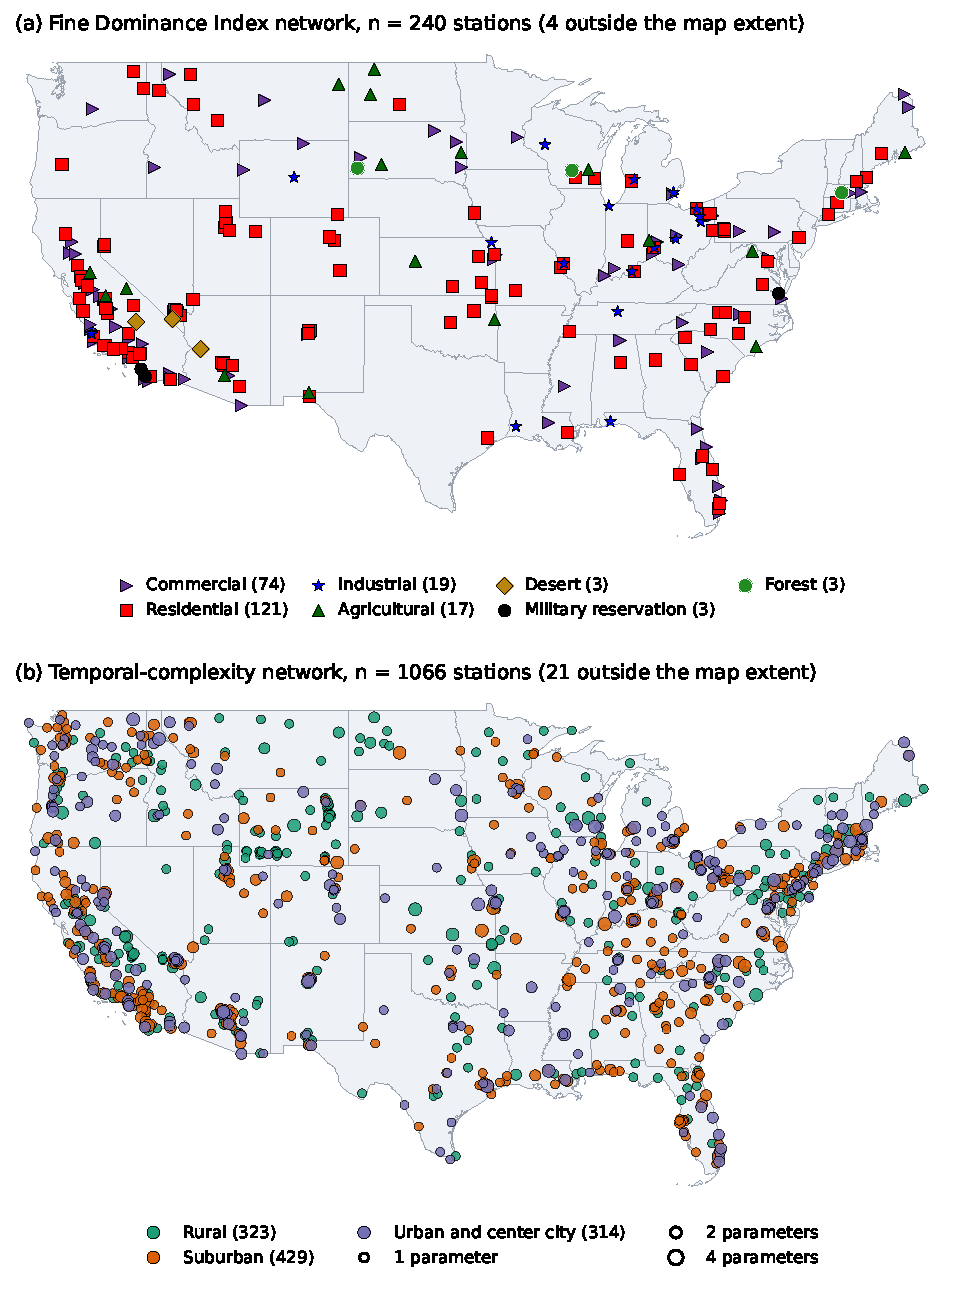
\includegraphics[width=0.86\linewidth]{figs/fig_station_map.pdf}
 \caption{Retained monitoring stations in the contiguous United States. (a) Fine--coarse (FDI) network ($n=240$), colored by land use; four stations in Alaska and Hawaii lie outside the map extent. (b) Temporal-complexity network ($n=1066$; 21 stations outside the map extent), colored by location setting; marker size indicates the number of parameters (PM$_{2.5}$ FRM/FEM, PM$_{2.5}$ non-FRM/FEM, PM$_{10}$, PM$_{c}$) that passed the completeness screen at each site.}
 \label{fig:stations_map}
\end{figure}

\subsection{Methods}

\subsubsection{Seasons and units of analysis}

Climatological seasons were defined by calendar months: winter (December--February), spring (March--May), summer (June--August), and autumn (September--November). For pooled seasonal summaries, each daily record inherits the season of its date. For analyses that require contiguous periods or year-specific units, we used season--years in which December is assigned to the following winter; thus, winter 2023 spans January--February 2023, winter 2024 spans December 2023--February 2024, and December 2025, which belongs to winter 2026, is not used. Daily values from the same monitor are serially correlated, so treating them as independent replicates inflates the significance of between-group tests \citep{Hurlbert1984, SierraPorta2026}. All hypothesis tests are therefore carried out on station-level units (station--season--year means for the fine--coarse layer and station medians for the complexity layer), whereas daily values are used only for descriptive distributions.

\subsubsection{Fine Dominance Index}

For each station-day with positive PM$_{2.5}$ and PM$_{10}$, we computed three ratios that capture complementary aspects of the fine--coarse partition \citep{Fan2021},
\begin{equation}
r_{12}=\frac{\mathrm{PM}_{2.5}}{\mathrm{PM}_{10}},\qquad
r_{21}=\frac{\mathrm{PM}_{10}}{\mathrm{PM}_{2.5}},\qquad
r_{0}=\frac{\mathrm{PM}_{10}-\mathrm{PM}_{2.5}}{\mathrm{PM}_{10}+\mathrm{PM}_{2.5}}\,,
\end{equation}
together with the per-sample Fine Dominance Index (FDI),
\begin{equation}
\mathrm{FDI}=\frac{\mathrm{PM}_{2.5}}{\mathrm{PM}_{10}}\,(1-r_{0})=\frac{2\,r_{12}^{2}}{1+r_{12}}\,,
\label{eq:fdi}
\end{equation}
which increases with fine-particle dominance. Because PM$_{2.5}$ is a subset of PM$_{10}$, days with PM$_{2.5}>$ PM$_{10}$ are physically inconsistent and reflect instrument differences or measurement uncertainty; they represent 1.6\% of the station-days with positive values and were excluded. With $0<r_{12}\le 1$, the FDI is bounded in $(0,1]$ and $r_0$ in $[0,1)$, so that neither index is affected by the near-zero denominators that make unbounded ratios heavy-tailed. The final fine--coarse dataset contains 241{,}664 station-days. Equation~(\ref{eq:fdi}) shows that the FDI is a monotone and convex transformation of $r_{12}$: it preserves the ranking of days while expanding differences among fine-dominated days, which is why rank-based tests on daily FDI, $r_{12}$, $r_{21}$, and $r_0$ are equivalent and only the FDI is reported.

\subsubsection{Cell-wise fingerprints and the composite index IFS}

For interpretability across contexts, observations were summarized in cells defined by the cross of land use, location setting, and season (56 populated cells). Within each cell we computed the mean of the FDI ($\overline{\mathrm{FDI}}$), the mean of $r_0$ ($\overline{r_0}$), and the skewness and excess kurtosis of $r_0$ (Fisher definitions). To provide a single fingerprint per cell, we built the composite index
\begin{equation}
\mathrm{IFS} \;=\; w_{\mathrm{FDI}}\;z\!\big(\overline{\mathrm{FDI}}\big)
 \;+\; w_{r_0}\;z\!\big(\overline{r_{0}}\big)
 \;+\; w_{\mathrm{skew}}\;z\!\big(\mathrm{skew}(r_{0})\big)
 \;+\; w_{\mathrm{kurt}}\;z\!\big(\mathrm{kurt}(r_{0})\big)\,,
\end{equation}
where $z(\cdot)$ denotes $z$-scores computed across all populated cells, and $w_{\mathrm{FDI}}=1.5$, $w_{r_0}=-1.0$, $w_{\mathrm{skew}}=-0.5$, and $w_{\mathrm{kurt}}=-0.5$. The weighting emphasizes fine dominance via $\overline{\mathrm{FDI}}$, penalizes coarse dominance via $\overline{r_0}$, and assigns a modest penalty to right-skewed, heavy-tailed $r_0$ distributions, which signal episodic coarse bursts. Because the components are standardized across cells, the IFS is on a $z$-scale: values near zero reflect network-average behavior, positive values indicate cells that are more fine-dominated than the network average with relatively muted coarse bursts, and negative values indicate comparatively coarse-dominated or bursty regimes.

Uncertainty in $\overline{\mathrm{FDI}}$ was quantified with a station-block bootstrap ($B=2000$) that resamples whole stations within each cell and therefore preserves the serial dependence of daily data \citep{Efron1994}. A cell was flagged as thin when it contained fewer than three stations, fewer than 300 station-days, or a 95\% bootstrap interval wider than 0.15 FDI units; thin cells are hatched in the heatmaps and excluded from the ranked tables. Of the 56 populated cells, 38 are not thin.

The robustness of the IFS was evaluated against (i) a grid of $5^4=625$ weight combinations ($w_{\mathrm{FDI}}\in[1.0,2.0]$, $w_{r_0}\in[-1.5,-0.5]$, $w_{\mathrm{skew}},w_{\mathrm{kurt}}\in[-1.0,0]$); (ii) named alternatives, including equal weights, location terms only, shape terms with a positive sign, and the mean FDI alone; (iii) the first principal component of the four standardized features; (iv) a stricter completeness threshold of 90\% (987 days); (v) the retention of days with PM$_{2.5}>$ PM$_{10}$ after capping $r_{12}$ at 1; (vi) alternative thin-cell criteria; and (vii) a separate recomputation for each season--year. Agreement with the nominal ranking of non-thin cells is reported as Kendall's $\tau$ and as the overlap of the top-10 and bottom-10 league tables.

\subsubsection{Formal contrasts}

Land uses were compared within each location setting and season on station--season--year means of the FDI, computed from units with at least 45 ratio days. Kruskal--Wallis omnibus tests \citep{Kruskal1952, Lachenbruch1991, MacFarland2016} included land uses with at least three stations, and the resulting family of omnibus tests (12 strata $\times$ four variables: FDI, $r_0$, PM$_{2.5}$, and PM$_{10}$) was adjusted with the Holm procedure \citep{Holm1979}. The omnibus effect size is reported as $\varepsilon^2=H/(n-1)$ \citep{Kelley1935}. Pairwise post hoc contrasts used two-sided Mann--Whitney tests \citep{Mann1947, Nachar2008} with Holm correction within each stratum, and magnitudes were summarized with Cliff's $\delta$ \citep{Cliff1993, Meissel2024}, interpreting $|\delta|<0.147$ as negligible, $0.147\le|\delta|<0.33$ as small, $0.33\le|\delta|<0.474$ as medium, and $|\delta|\ge0.474$ as large \citep{Romano2006}. The seasonal contrast within stations was evaluated with the Friedman test on station-level seasonal means of the FDI \citep{Friedman1937}, with Kendall's $W$ as effect size \citep{Kendall1939}.

\subsubsection{Temporal complexity of daily PM series}

For every station and parameter of the complexity network, the daily series was partitioned into season--year windows (12 windows per station). A window was analyzed when at least 75\% of its calendar days had data; gaps of up to three days were linearly interpolated, and longer gaps were left unfilled. Each window (on average 90 days) was standardized, and ties, which are frequent because PM$_{10}$ is reported with a resolution of 1\,\textmu g\,m$^{-3}$, were broken at random with a negligible jitter, since equal values otherwise bias ordinal-pattern statistics \citep{Zunino2017}. A total of 16{,}411 windows were analyzed (8664 for PM$_{2.5}$ FRM/FEM, 1936 for PM$_{2.5}$ non-FRM/FEM, 4782 for PM$_{10}$, and 1029 for PM$_{c}$).

The metrics, summarized in Table~\ref{tab:metrics}, follow established definitions. For ordinal patterns of embedding dimension $D$ and delay $\tau$ with probability distribution $P=\{p_i\}_{i=1}^{D!}$, the normalized permutation entropy is $H[P]=-\sum_i p_i\ln p_i/\ln D!$ \citep{Bandt2002}, and the Jensen--Shannon statistical complexity is $C_{JS}[P]=Q_J[P,P_e]\,H[P]$, where $Q_J$ is the normalized Jensen--Shannon divergence between $P$ and the uniform distribution $P_e$ \citep{Lamberti2004, Rosso2007}. Sample entropy is $-\ln(A/B)$, where $B$ and $A$ count pairs of templates of length $m$ and $m+1$ that match within a tolerance $r$ \citep{Richman2000}. SVD entropy is the normalized Shannon entropy of the singular values of the embedding matrix \citep{Roberts1999}; the Higuchi fractal dimension is the slope of the log--log relation between curve length and scale \citep{Higuchi1988}; and the correlation dimension $D_2$ is the scaling exponent of the Grassberger--Procaccia correlation sum \citep{Grassberger1983}, estimated by RANSAC regression with a fixed random seed for reproducibility. Skewness and excess kurtosis of the concentrations describe the asymmetry and tail weight of each window. Permutation entropy, SVD entropy, and the Higuchi dimension were computed with \texttt{antropy} (0.2.2), sample entropy and the correlation dimension with \texttt{nolds} (0.6.3), and the statistical complexity with our own implementation of the Jensen--Shannon formulation.

\begin{table*}[!htbp]
\centering
\footnotesize
\caption{Temporal-complexity metrics computed for each station--parameter--season--year window. The full-period ordinal analysis uses $D=4$ on the complete 2023--2025 record of each station.}
\label{tab:metrics}
\begin{tabular}{p{3.3cm}p{4.4cm}p{1.6cm}p{5.0cm}}
\toprule
\textbf{Metric} & \textbf{Settings} & \textbf{Range} & \textbf{High values indicate} \\
\midrule
Permutation entropy $H$ & Ordinal patterns, $D=3$ (windows) or $D=4$ (full period), $\tau=1$ day & $[0,1]$ & Ordinal sequences closer to uncorrelated noise \\
Statistical complexity $C_{JS}$ & Same ordinal distribution as $H$ & $[0,C_{\max}(H)]$ & Structured, correlated dynamics that are neither fully ordered nor random \\
Sample entropy & $m=2$, $r=0.2\times$SD & $\geq 0$ & Amplitude irregularity (few repeated templates) \\
SVD entropy & Embedding order 3, $\tau=1$ day & $[0,1]$ & More independent components in the embedded trajectory \\
Higuchi fractal dimension & $k_{\max}=10$ & $[1,2]$ & Rougher trajectories (1.5 for Brownian motion, 2 for white noise) \\
Correlation dimension $D_2$ & Embedding dimension 2 & $[0,2]$ & Space-filling of the reconstructed state space (bounded by the embedding) \\
Skewness, excess kurtosis & Fisher definitions & $\mathbb{R}$ & Asymmetric, heavy-tailed (bursty) concentration distributions \\
\bottomrule
\end{tabular}
\end{table*}

The temporal structure of each window was tested against 199 shuffled surrogates, which preserve the distribution of values but destroy temporal order \citep{Theiler1992}; a window is considered ordered when its permutation entropy lies below the surrogate distribution at the 5\% level. Because $D=3$ (six patterns) is appropriate for windows of about 90 days but provides a coarse description of the complexity--entropy plane, we also computed $H$ and $C_{JS}$ with $D=4$ (24 patterns) from the complete 2023--2025 record of each station, counting ordinal patterns only within contiguous data segments, and compared them with the bounds $C_{\min}(H)$ and $C_{\max}(H)$ of the plane \citep{Martin2006} and with 99 shuffled surrogates per station.

Window-level metrics were summarized by their median per station (and per station and season). Differences among land uses and among location settings were tested with Kruskal--Wallis tests on station medians (groups with at least five stations; $\varepsilon^2$ as effect size), seasonal differences within stations with Friedman tests (Kendall's $W$), and differences between size fractions measured at the same site with Wilcoxon signed-rank tests \citep{Wilcoxon1945}, summarized by the matched-pairs rank-biserial correlation $r_{rb}$ \citep{Kerby2014}. Holm corrections were applied within each family of tests. Redundancy among metrics was assessed with Spearman correlations across all windows, and the persistence of station rankings with Spearman correlations between years. Finally, the PM$_{2.5}$ FRM/FEM stations were grouped by Ward's hierarchical clustering \citep{Ward1963} of the standardized medians of four non-redundant dynamical metrics ($H$, sample entropy, SVD entropy, and Higuchi dimension), with $k=3$; $C_{JS}$ was omitted because it is a deterministic function of $H$ for $D=3$, and $D_2$ because it is the least stable estimate. Cluster quality was assessed with the silhouette width and by reclustering 200 random subsamples of 80\% of the stations, and agreement between clusters and land use or location setting was measured with the adjusted Rand index \citep{Hubert1985} and Cram\'er's $V$.

\subsubsection{Linking the fine--coarse partition and temporal complexity}

At the 240 stations of the fine--coarse network, the station mean FDI was correlated with the station-median complexity metrics of the collocated PM$_{2.5}$ FRM/FEM and PM$_{10}$ series using Spearman's $\rho_s$, with Holm correction. Because both the size partition and the dynamics vary regionally, we also report partial Spearman correlations controlling for latitude and longitude.

\subsubsection{Software and reproducibility}

All analyses were performed in Python 3.13 with \texttt{pandas}, \texttt{numpy}, \texttt{scipy}, \texttt{scikit-learn}, \texttt{matplotlib}, \texttt{antropy}, and \texttt{nolds}. The pipeline downloads the public EPA AirData files, applies the reduction and screening rules described above, and reproduces every table and figure of this article with fixed random seeds.

\section{Results and Discussion}\label{sec:results}
\subsection{Sample-level distributions of fine dominance}

Figure~\ref{fig:fdi_facets} displays the daily FDI by land use, location setting, and season under a common $y$-axis. The dominant feature is seasonal. Station-level FDI peaks in winter at 83\% of the monitors, with a network median of 0.35 in winter against 0.25 in spring, 0.23 in summer, and 0.24 in autumn (Friedman $\chi^2=301.6$, $p<0.001$, Kendall's $W=0.42$). The seasonal contrast is strongest in suburban ($W=0.49$) and urban ($W=0.43$) settings and weaker, though still significant, in rural settings ($W=0.29$). This pattern is consistent with shallow wintertime boundary layers, residential heating, and the accumulation of secondary fine aerosol during stagnation, and with the larger contribution of resuspended and wind-blown coarse particles in the warm and dry seasons \citep{Jandacka2024, Czernecki2021, Clements2016}.

\begin{figure}[!htbp]
  \centering
  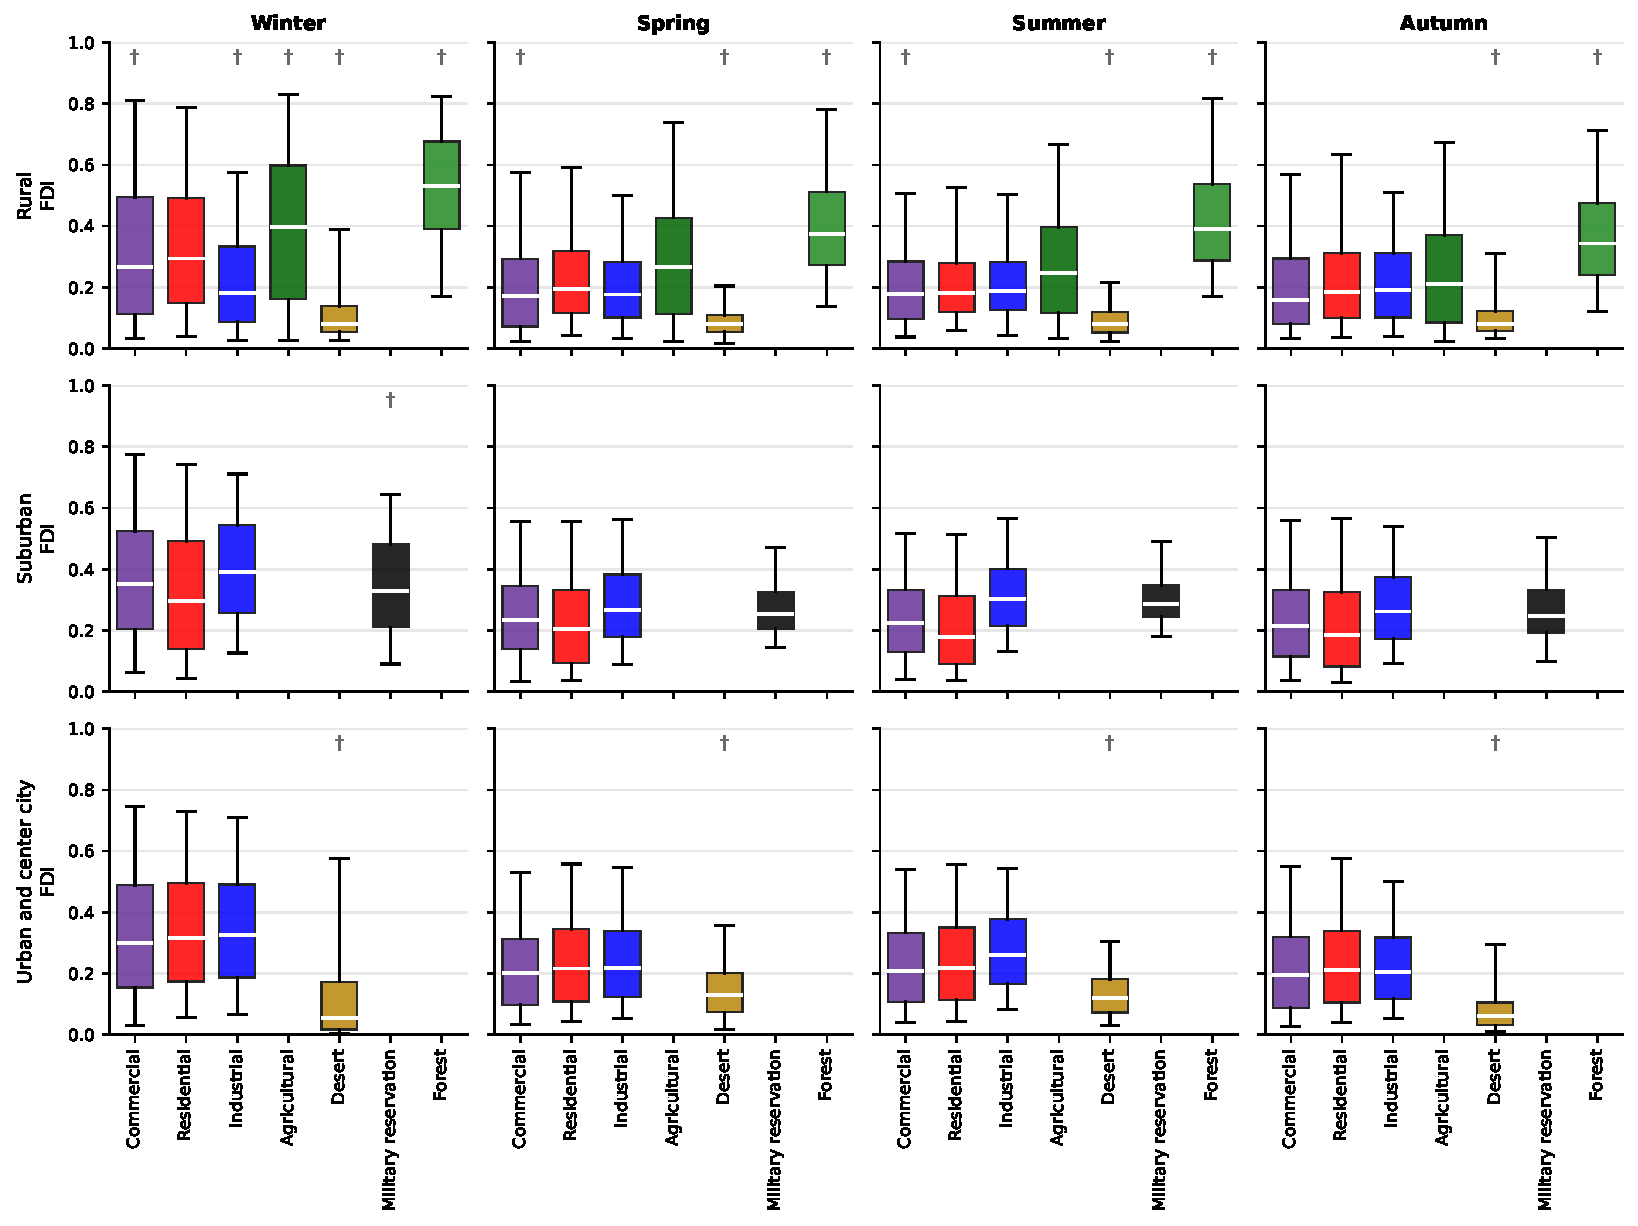
\includegraphics[width=\linewidth]{figs/fig_fdi_boxplots.pdf}
  \caption{Daily Fine Dominance Index (FDI) by land use, with location setting in rows and season in columns. Boxes show medians and interquartile ranges, and whiskers span the 5th--95th percentiles; values outside the whiskers are not drawn. All panels share the $y$-axis. Daggers (\dag) mark thin cells (fewer than three stations, fewer than 300 station-days, or a 95\% station-block bootstrap interval wider than 0.15). Larger FDI indicates stronger fine-particle dominance relative to coarse contributions.}
  \label{fig:fdi_facets}
\end{figure}

Within each setting and season, the distributions of commercial, residential, and industrial monitors overlap broadly, with interquartile ranges that share most of their extent. The clearest separations involve the less common classes. Rural forest monitors are the most fine-dominated in every season (median FDI between 0.34 and 0.53), as expected for sites with little local resuspension that are periodically affected by smoke. Desert monitors are the most coarse-dominated, with medians below 0.15 in every setting and season, which reflects persistent soil dust. Agricultural monitors show a wide winter distribution and moderate values in the rest of the year, in line with the seasonal contribution of secondary ammonium nitrate in agricultural regions \citep{Burns2023, Bell2007}. Higher FDI values point to combustion- and secondary-aerosol influence, whereas lower values indicate coarse dominance from resuspension or natural dust \citep{Liu2023, Xu2020}; within a given setting, the contrasts among classes plausibly reflect activity patterns and surface characteristics \citep{Wei2021, Clark2013}. Where distributions overlap, the overlap suggests mixed-source environments or within-class heterogeneity, which motivates the cell-wise summaries and formal tests that follow.

\subsection{Cell-wise seasonal fingerprints (IFS)}

Figure~\ref{fig:fdi_heatmaps} summarizes the composite IFS for each land use, location setting, and season under a common, zero-centered color scale. In suburban and urban settings, winter is the only season in which every built-environment class has a positive IFS (1.67--3.63), which identifies a coherent wintertime fine-dominance regime in commercial, residential, and industrial areas. Suburban industrial sites stand out with positive values in all seasons (1.11--3.63), and the three suburban military reservation sites are also fine-dominated outside winter. In rural settings, residential sites follow the winter pattern (1.94), agricultural sites are mildly positive in spring and summer (1.04 and 0.71), and industrial sites are the most coarse-dominated non-thin cells of the network in spring, summer, and autumn ($-1.25$ to $-0.98$). The extremes of the IFS scale correspond to thin cells: forest sites are strongly positive in all seasons (2.55--4.84), and desert sites are strongly negative in all seasons and settings ($-5.65$ to $-3.14$), in agreement with the boxplots but based on only one to three stations.

\begin{figure}[!htbp]
  \centering
  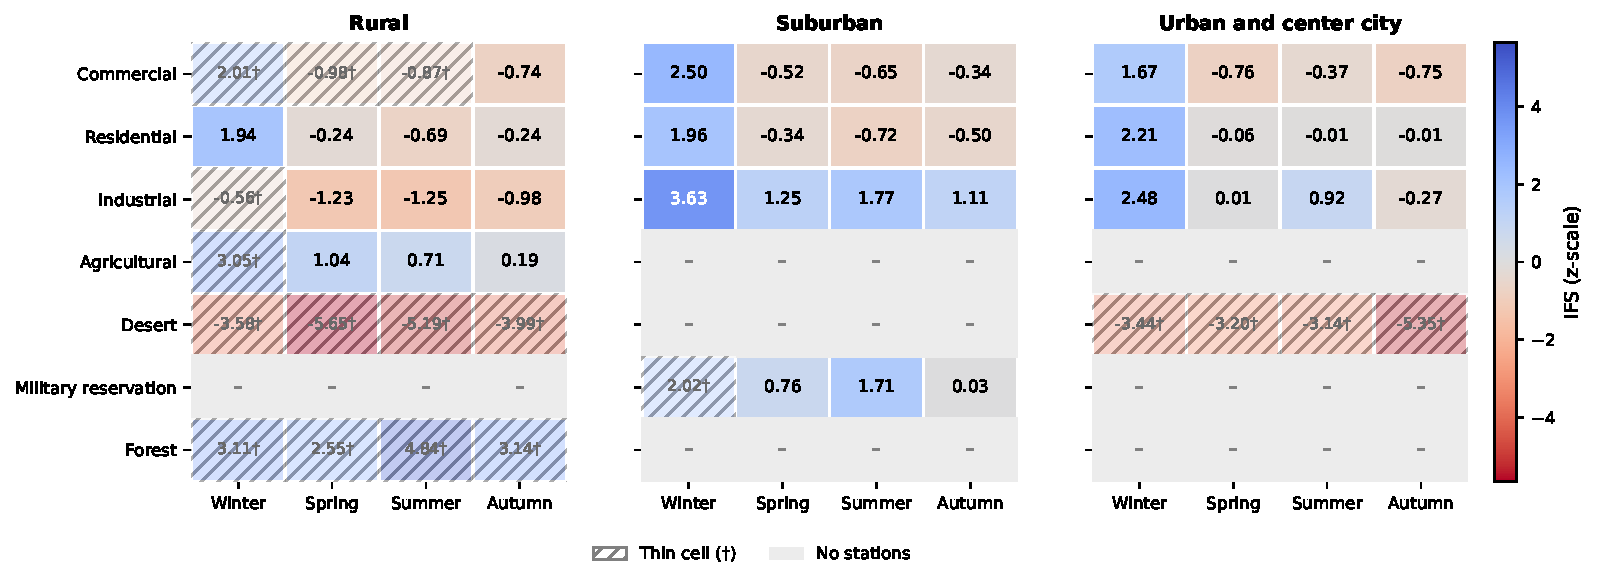
\includegraphics[width=\linewidth]{figs/fig_ifs_heatmap.pdf}
  \caption{Cell-wise seasonal fingerprints given by the standardized composite index (IFS), by land use (rows) and season (columns), in three panels by location setting. The color scale is centered at zero and common to all panels. Hatched cells marked with a dagger (\dag) are thin and are excluded from the ranked tables; grey cells contain no stations. Positive values indicate stronger fine-particle dominance and more muted coarse bursts than the network-wide average across all cells.}
  \label{fig:fdi_heatmaps}
\end{figure}

Two points guide the interpretation. First, because the IFS is standardized across all cells and seasons, positive cells mark regimes that are more fine-dominated than the network-wide average, and negative cells mark comparatively coarse-dominated or bursty regimes; the values are therefore relative and should be read together with the physically interpretable FDI means. Second, outlying values often correspond to sparse classes or to seasons affected by episodic dust or smoke; when the number of stations is small or the bootstrap interval is wide, the corresponding cells are flagged rather than ranked.

\subsection{Formal contrasts and ranked hotspots/coldspots}

Table~\ref{tab:hotcold_overall} ranks the non-thin cells by IFS. Seven of the ten hotspots are winter cells in built environments (suburban industrial, suburban commercial, urban industrial, urban residential, suburban residential, rural residential, and urban commercial), with mean FDI between 0.33 and 0.40, while the remaining three are suburban industrial and military reservation cells in summer and spring. The coldspots are dominated by rural industrial cells outside winter and by spring, summer, and autumn cells of commercial and residential sites, with mean FDI between 0.21 and 0.26 and mean $r_0$ close to 0.5. The skewness and kurtosis of $r_0$ are moderate in all ranked cells ($|\mathrm{skew}|\le0.6$, $|\mathrm{kurt}|\le0.8$), which confirms that, once physically inconsistent days are removed, the ranking is driven by the location of the fine--coarse partition rather than by tail artifacts.

\begin{table*}[!htbp]
\centering
\scriptsize
\caption{Top 10 hotspots (highest IFS) and bottom 10 coldspots (lowest IFS) among the 38 non-thin cells. Columns report the cell mean of the FDI with its 95\% station-block bootstrap interval, the number of contributing station-days ($n$) and stations ($n_{\mathrm{st}}$), the composite index (IFS), and the mean, skewness, and excess kurtosis of $r_0$. Thin cells, including all desert and forest cells, are shown in Fig.~\ref{fig:fdi_heatmaps}.}
\label{tab:hotcold_overall}
\begin{tabular}{lllcccrrccc}
\toprule
\multicolumn{11}{c}{\textbf{Top 10 hotspots (highest IFS): most fine-dominated}} \\
\midrule
\textbf{Land use} & \textbf{Location setting} & \textbf{Season} & \textbf{$\overline{\mathrm{FDI}}$} & \textbf{95\% CI} & \textbf{$n$} & \textbf{$n_{\mathrm{st}}$} & \textbf{IFS} & \textbf{Mean $r_0$} & \textbf{Skew $r_0$} & \textbf{Kurt $r_0$} \\
\midrule
Industrial & Suburban & Winter & 0.40 & [0.36, 0.46] & 1653 & 7 & 3.63 & 0.31 & 0.49 & $-0.31$ \\
Commercial & Suburban & Winter & 0.38 & [0.32, 0.43] & 5262 & 22 & 2.50 & 0.34 & 0.59 & 0.06 \\
Industrial & Urban and center city & Winter & 0.35 & [0.31, 0.40] & 1788 & 8 & 2.48 & 0.36 & 0.36 & $-0.54$ \\
Residential & Urban and center city & Winter & 0.35 & [0.31, 0.38] & 10402 & 42 & 2.21 & 0.37 & 0.39 & $-0.44$ \\
Residential & Suburban & Winter & 0.33 & [0.30, 0.36] & 17343 & 70 & 1.96 & 0.39 & 0.31 & $-0.75$ \\
Residential & Rural & Winter & 0.34 & [0.28, 0.42] & 2202 & 9 & 1.94 & 0.38 & 0.33 & $-0.47$ \\
Industrial & Suburban & Summer & 0.32 & [0.28, 0.35] & 1867 & 7 & 1.77 & 0.36 & 0.22 & $-0.23$ \\
Military reservation & Suburban & Summer & 0.30 & [0.27, 0.37] & 795 & 3 & 1.71 & 0.37 & $-0.30$ & 0.50 \\
Commercial & Urban and center city & Winter & 0.33 & [0.29, 0.37] & 11229 & 46 & 1.67 & 0.39 & 0.48 & $-0.43$ \\
Industrial & Suburban & Spring & 0.29 & [0.25, 0.33] & 1776 & 7 & 1.25 & 0.39 & 0.12 & $-0.53$ \\
\midrule
\multicolumn{11}{c}{\textbf{Bottom 10 coldspots (lowest IFS): most coarse-dominated}} \\
\midrule
\textbf{Land use} & \textbf{Location setting} & \textbf{Season} & \textbf{$\overline{\mathrm{FDI}}$} & \textbf{95\% CI} & \textbf{$n$} & \textbf{$n_{\mathrm{st}}$} & \textbf{IFS} & \textbf{Mean $r_0$} & \textbf{Skew $r_0$} & \textbf{Kurt $r_0$} \\
\midrule
Industrial & Rural & Summer & 0.22 & [0.20, 0.25] & 1009 & 4 & $-1.25$ & 0.47 & 0.10 & 0.40 \\
Industrial & Rural & Spring & 0.21 & [0.16, 0.27] & 1002 & 4 & $-1.23$ & 0.49 & $-0.04$ & $-0.04$ \\
Industrial & Rural & Autumn & 0.22 & [0.17, 0.29] & 933 & 4 & $-0.98$ & 0.47 & 0.18 & $-0.29$ \\
Commercial & Urban and center city & Spring & 0.23 & [0.20, 0.25] & 11535 & 46 & $-0.76$ & 0.47 & 0.13 & $-0.47$ \\
Commercial & Urban and center city & Autumn & 0.23 & [0.20, 0.25] & 11792 & 46 & $-0.75$ & 0.48 & 0.09 & $-0.55$ \\
Commercial & Rural & Autumn & 0.21 & [0.14, 0.28] & 1495 & 6 & $-0.74$ & 0.50 & $-0.35$ & $-0.50$ \\
Residential & Suburban & Summer & 0.22 & [0.19, 0.24] & 18245 & 70 & $-0.72$ & 0.48 & $-0.04$ & $-0.69$ \\
Residential & Rural & Summer & 0.22 & [0.18, 0.27] & 2291 & 9 & $-0.69$ & 0.47 & $-0.35$ & 0.28 \\
Commercial & Suburban & Summer & 0.24 & [0.20, 0.29] & 5580 & 22 & $-0.65$ & 0.45 & 0.40 & $-0.21$ \\
Commercial & Suburban & Spring & 0.26 & [0.22, 0.29] & 5278 & 22 & $-0.52$ & 0.44 & 0.44 & 0.09 \\
\bottomrule
\end{tabular}
\end{table*}

For context-specific decisions, Table~\ref{tab:hotcold_by_loc} lists, within each location setting, the non-thin cells with positive IFS (up to five). In rural areas, the residential winter cell leads, followed by agricultural cells in spring, summer, and autumn, consistent with secondary fine aerosol from agricultural ammonia and with wintertime residential combustion \citep{Burns2023, Jandacka2024}. In suburban areas, all built environments are fine-dominated in winter, and industrial and military reservation sites remain so in summer. In urban and center-city settings, the industrial, residential, and commercial winter cells lead, and only industrial sites retain positive values outside winter, suggesting a combustion-related fine component that persists across seasons near industrial sources \citep{Cummings2021}.

\begin{table*}[!htbp]
\centering
\scriptsize
\caption{Non-thin cells with positive IFS within each location setting (up to five per setting). Columns as in Table~\ref{tab:hotcold_overall}.}
\label{tab:hotcold_by_loc}
\begin{tabular}{lllcccrrccc}
\toprule
\textbf{Land use} & \textbf{Location setting} & \textbf{Season} & \textbf{$\overline{\mathrm{FDI}}$} & \textbf{95\% CI} & \textbf{$n$} & \textbf{$n_{\mathrm{st}}$} & \textbf{IFS} & \textbf{Mean $r_0$} & \textbf{Skew $r_0$} & \textbf{Kurt $r_0$} \\
\midrule
\multicolumn{11}{l}{\textbf{Rural}} \\
Residential & Rural & Winter & 0.34 & [0.28, 0.42] & 2202 & 9 & 1.94 & 0.38 & 0.33 & $-0.47$ \\
Agricultural & Rural & Spring & 0.30 & [0.23, 0.36] & 4122 & 17 & 1.04 & 0.42 & 0.27 & $-0.70$ \\
Agricultural & Rural & Summer & 0.28 & [0.22, 0.34] & 4397 & 17 & 0.71 & 0.43 & 0.20 & $-0.66$ \\
Agricultural & Rural & Autumn & 0.26 & [0.20, 0.31] & 4304 & 17 & 0.19 & 0.46 & 0.04 & $-0.83$ \\
\midrule
\multicolumn{11}{l}{\textbf{Suburban}} \\
Industrial & Suburban & Winter & 0.40 & [0.36, 0.46] & 1653 & 7 & 3.63 & 0.31 & 0.49 & $-0.31$ \\
Commercial & Suburban & Winter & 0.38 & [0.32, 0.43] & 5262 & 22 & 2.50 & 0.34 & 0.59 & 0.06 \\
Residential & Suburban & Winter & 0.33 & [0.30, 0.36] & 17343 & 70 & 1.96 & 0.39 & 0.31 & $-0.75$ \\
Industrial & Suburban & Summer & 0.32 & [0.28, 0.35] & 1867 & 7 & 1.77 & 0.36 & 0.22 & $-0.23$ \\
Military reservation & Suburban & Summer & 0.30 & [0.27, 0.37] & 795 & 3 & 1.71 & 0.37 & $-0.30$ & 0.50 \\
\midrule
\multicolumn{11}{l}{\textbf{Urban and center city}} \\
Industrial & Urban and center city & Winter & 0.35 & [0.31, 0.40] & 1788 & 8 & 2.48 & 0.36 & 0.36 & $-0.54$ \\
Residential & Urban and center city & Winter & 0.35 & [0.31, 0.38] & 10402 & 42 & 2.21 & 0.37 & 0.39 & $-0.44$ \\
Commercial & Urban and center city & Winter & 0.33 & [0.29, 0.37] & 11229 & 46 & 1.67 & 0.39 & 0.48 & $-0.43$ \\
Industrial & Urban and center city & Summer & 0.28 & [0.22, 0.34] & 1881 & 8 & 0.92 & 0.40 & 0.19 & $-0.42$ \\
Industrial & Urban and center city & Spring & 0.25 & [0.20, 0.29] & 1875 & 8 & 0.01 & 0.44 & 0.05 & $-0.42$ \\
\bottomrule
\end{tabular}
\end{table*}

Rankings alone do not quantify separations between land uses, and Table~\ref{tab:fdi_contrasts} reports the formal contrasts on station--season--year units. After Holm correction across the 48 omnibus tests, land-use differences in the FDI are significant only in rural summer ($\varepsilon^2=0.17$, $p_{\mathrm{Holm}}=0.024$) and suburban summer ($\varepsilon^2=0.06$, $p_{\mathrm{Holm}}=0.014$). The largest effects involve forest sites, whose FDI exceeds that of industrial, commercial, and residential rural sites in summer ($\delta=0.88$--$0.94$, large) and autumn ($\delta=0.77$--$0.80$), and suburban industrial sites, which exceed residential ($\delta=0.49$, large) and commercial ($\delta=0.43$, medium) sites in summer. In urban and center-city settings, the effect sizes are negligible to small ($\varepsilon^2\le0.012$; $|\delta|\le0.24$), so that commercial, residential, and industrial urban monitors share essentially the same fine--coarse partition in every season. This conclusion differs from what daily-level tests would suggest, because with tens of thousands of serially correlated days almost any difference becomes ``significant''; it agrees with the companion station--season analysis, in which land-use contrasts were generally modest relative to seasonality \citep{SierraPorta2026}. For PM$_{2.5}$ concentrations, in contrast, land-use differences reach significance in urban summer ($\varepsilon^2=0.09$, $p_{\mathrm{Holm}}<0.001$) and spring ($\varepsilon^2=0.05$, $p_{\mathrm{Holm}}=0.024$), which indicates that land use modulates the level of fine particles more than their share of PM$_{10}$.

\begin{table*}[!htbp]
\centering
\scriptsize
\caption{Land-use contrasts of the FDI within each location setting and season, computed on station--season--year means. Groups list the land uses with at least three stations (number of stations in parentheses; Com.\ = commercial, Res.\ = residential, Ind.\ = industrial, Agr.\ = agricultural, For.\ = forest, Mil.\ = military reservation). $H$ and $\varepsilon^2$ refer to the Kruskal--Wallis test, with Holm adjustment across the 48 omnibus tests; the last three columns give the pairwise contrast with the largest Cliff's $\delta$ and its Holm-adjusted Mann--Whitney $p$-value.}
\label{tab:fdi_contrasts}
\setlength{\tabcolsep}{3pt}
\begin{tabular}{ll>{\raggedright\arraybackslash}p{3.7cm}rrrrlrr}
\toprule
\textbf{Location setting} & \textbf{Season} & \textbf{Groups} & \textbf{Units} & \textbf{$H$} & \textbf{$\varepsilon^2$} & \textbf{$p_{\mathrm{Holm}}$} & \textbf{Largest contrast} & \textbf{$\delta$} & \textbf{$p_{\mathrm{Holm}}$} \\
\midrule
Rural & Winter & Com.\,(6), Res.\,(9), Ind.\,(4), Agr.\,(16) & 89 & 12.43 & 0.141 & 0.235 & Agricultural $>$ Industrial & 0.57 & 0.035 \\
Rural & Spring & Com.\,(6), Res.\,(9), Ind.\,(4), Agr.\,(17) & 103 & 9.45 & 0.093 & 0.667 & Agricultural $>$ Industrial & 0.40 & 0.168 \\
Rural & Summer & Com.\,(6), Res.\,(9), Ind.\,(4), Agr.\,(17), For.\,(3) & 117 & 19.64 & 0.169 & 0.024 & Forest $>$ Industrial & 0.94 & 0.003 \\
Rural & Autumn & Com.\,(6), Res.\,(9), Ind.\,(4), Agr.\,(17), For.\,(3) & 111 & 13.71 & 0.125 & 0.298 & Forest $>$ Industrial & 0.80 & 0.024 \\
Suburban & Winter & Com.\,(22), Res.\,(70), Ind.\,(7), Mil.\,(3) & 281 & 5.05 & 0.018 & 1.000 & Industrial $>$ Military res. & 0.32 & 0.865 \\
Suburban & Spring & Com.\,(22), Res.\,(70), Ind.\,(7), Mil.\,(3) & 295 & 5.77 & 0.020 & 1.000 & Industrial $>$ Residential & 0.29 & 0.211 \\
Suburban & Summer & Com.\,(22), Res.\,(70), Ind.\,(7), Mil.\,(3) & 301 & 18.69 & 0.062 & 0.014 & Industrial $>$ Residential & 0.49 & 0.001 \\
Suburban & Autumn & Com.\,(22), Res.\,(70), Ind.\,(7), Mil.\,(3) & 302 & 7.26 & 0.024 & 1.000 & Industrial $>$ Residential & 0.31 & 0.116 \\
Urban and center city & Winter & Com.\,(46), Res.\,(42), Ind.\,(8) & 259 & 0.97 & 0.004 & 1.000 & Residential $>$ Commercial & 0.07 & 1.000 \\
Urban and center city & Spring & Com.\,(46), Res.\,(42), Ind.\,(8) & 277 & 2.54 & 0.009 & 1.000 & Industrial $>$ Commercial & 0.15 & 0.524 \\
Urban and center city & Summer & Com.\,(46), Res.\,(42), Ind.\,(8) & 280 & 3.31 & 0.012 & 1.000 & Industrial $>$ Commercial & 0.24 & 0.201 \\
Urban and center city & Autumn & Com.\,(46), Res.\,(42), Ind.\,(8) & 286 & 1.66 & 0.006 & 1.000 & Residential $>$ Commercial & 0.09 & 0.600 \\
\bottomrule
\end{tabular}
\end{table*}

\subsection{Robustness of the fine--coarse fingerprints}

Table~\ref{tab:ifs_robustness} summarizes the sensitivity of the IFS ranking. Across the 625 weight combinations, the median Kendall's $\tau$ with the nominal ranking is 0.88 (minimum 0.70), and the median overlap of the top-10 list is complete (minimum 0.8), whereas the bottom of the ranking, where cells are less separated, is somewhat more sensitive (median overlap 0.8, minimum 0.7). The first principal component of the standardized features explains 71\% of their variance and correlates strongly with the IFS (Spearman $\rho=0.88$); its loadings are dominated by the mean FDI ($+0.66$) and the mean $r_0$ ($-0.59$), which shows that the index is aligned with the main fine--coarse axis of the data. The component also loads positively on the skewness of $r_0$ ($+0.46$), because the bounded $r_0$ has more room for right-tail excursions where it is low, whereas the IFS deliberately penalizes those excursions as coarse bursts; consistently, the variant with positive shape weights yields the lowest agreement ($\tau=0.72$). A stricter 90\% completeness threshold (199 stations) and the retention of physically inconsistent days leave the ranking largely unchanged ($\tau=0.90$ and $0.89$; Spearman $\rho=0.98$ in both cases).

\begin{table}[!htbp]
\centering
\footnotesize
\caption{Robustness of the IFS ranking. Kendall's $\tau$ compares the nominal and alternative IFS values over the cells that are not thin under either specification; the overlaps compare each specification's own top-10 and bottom-10 lists with the nominal lists.}
\label{tab:ifs_robustness}
\begin{tabular}{p{6.6cm}ccc}
\toprule
\textbf{Specification} & \textbf{Kendall's $\tau$} & \textbf{Top-10 overlap} & \textbf{Bottom-10 overlap} \\
\midrule
Weight grid (625 combinations), median [minimum] & 0.88 [0.70] & 1.0 [0.8] & 0.8 [0.7] \\
Equal weights $(1,-1,-1,-1)$ & 0.80 & 0.9 & 0.8 \\
Location terms only $(1.5,-1,0,0)$ & 0.84 & 1.0 & 0.8 \\
Shape terms with positive sign $(1.5,-1,+0.5,+0.5)$ & 0.72 & 0.9 & 0.6 \\
Mean FDI only & 0.86 & 0.9 & 0.8 \\
First principal component (71\% of variance) & 0.71 & 0.9 & 0.6 \\
\midrule
Completeness $\geq$90\% (199 stations) & 0.90 & 0.9 & 0.9 \\
Days with PM$_{2.5}>$ PM$_{10}$ retained ($r_{12}$ capped at 1) & 0.89 & 1.0 & 0.9 \\
Thin-cell interval tolerance 0.10 (25 non-thin cells) & 1.00 & 0.6 & 0.7 \\
No interval criterion for thin cells (48 non-thin cells) & 1.00 & 0.4 & 0.8 \\
\midrule
Season--year 2023 only & 0.75 & 0.6 & 0.7 \\
Season--year 2024 only & 0.79 & 0.8 & 0.6 \\
Season--year 2025 only & 0.81 & 0.7 & 0.7 \\
\bottomrule
\end{tabular}
\end{table}

The composition of the league tables is more sensitive to the treatment of thin cells than to the weighting. A tighter interval tolerance removes several winter hotspots with heterogeneous stations, whereas dropping the interval criterion lets sparse forest and agricultural winter cells enter the top of the ranking; in both cases the values of the IFS are unchanged ($\tau=1$), so that only the eligibility of cells differs. Recomputing the IFS separately for each season--year reproduces the nominal ranking with Spearman correlations of 0.91--0.93 ($\tau=0.75$--$0.81$). Winter cells of built environments occupy 7 and 6 of the top-10 positions in 2024 and 2025, respectively, but only 4 in 2023, when the winter season covers only January and February and the summer was affected by smoke from the record Canadian wildfires \citep{Wang2024}; in that year, summer and spring cells of suburban and urban industrial sites rank higher. The qualitative hierarchy (wintertime fine dominance in built environments, coarse dominance in rural industrial and desert settings) is therefore robust, whereas the exact order of mid-ranked cells should not be over-interpreted.

\subsection{Temporal complexity of daily PM series}

Table~\ref{tab:complexity_summary} summarizes the complexity metrics by parameter. All size fractions occupy the high-entropy, low-complexity region of the complexity--entropy plane (Fig.~\ref{fig:cecp}): with $D=4$ over the full record, the median permutation entropy ranges from 0.955 for PM$_{2.5}$ FRM/FEM to 0.964 for PM$_{c}$, and the statistical complexity from 0.055 to 0.044. Daily PM concentrations therefore behave as strongly stochastic, correlated-noise processes, as also reported for most environmental time series \citep{Amato2020, Nikolopoulos2021, Ribeiro2017}. They are not random, however: shuffled surrogates reach $H=0.997$ and $C_{JS}=0.004$, and the full-period entropy of 99.8--100\% of the stations lies significantly below its surrogate distribution. Within individual seasonal windows, where only about 90 values are available, the ordinal structure is detectable in 48--59\% of the windows, with the highest rates in summer for PM$_{2.5}$ FRM/FEM (70\%) and the lowest in winter for all parameters (36--41\%). Day-to-day winter variability is thus closer to random, consistent with the rapid alternation of stagnation and ventilation imposed by synoptic systems, whereas summer variability is more persistent.

\begin{table*}[!htbp]
\centering
\footnotesize
\caption{Temporal-complexity metrics by parameter: medians [interquartile ranges] across season--year windows ($D=3$) and across stations for the full-period ordinal analysis ($D=4$). Ordered windows are those whose permutation entropy lies below the 5th percentile of 199 shuffled surrogates.}
\label{tab:complexity_summary}
\setlength{\tabcolsep}{4pt}
\begin{tabular}{lcccc}
\toprule
 & \textbf{PM$_{2.5}$ FRM/FEM} & \textbf{PM$_{2.5}$ non-FRM/FEM} & \textbf{PM$_{10}$} & \textbf{PM$_{c}$} \\
\midrule
Stations & 751 & 171 & 420 & 91 \\
Season--year windows & 8664 & 1936 & 4782 & 1029 \\
Ordered windows (\%) & 58.1 & 58.8 & 49.9 & 47.8 \\
\midrule
Permutation entropy $H$ ($D=3$) & 0.965 [0.949, 0.978] & 0.964 [0.948, 0.977] & 0.969 [0.954, 0.981] & 0.970 [0.955, 0.982] \\
Statistical complexity $C_{JS}$ ($D=3$) & 0.033 [0.021, 0.047] & 0.033 [0.022, 0.048] & 0.029 [0.018, 0.043] & 0.028 [0.018, 0.041] \\
Sample entropy & 1.61 [1.33, 1.88] & 1.50 [1.16, 1.79] & 1.51 [1.21, 1.80] & 1.58 [1.28, 1.82] \\
SVD entropy & 0.943 [0.916, 0.964] & 0.929 [0.901, 0.956] & 0.951 [0.922, 0.975] & 0.954 [0.929, 0.974] \\
Higuchi fractal dimension & 1.84 [1.78, 1.89] & 1.83 [1.76, 1.88] & 1.85 [1.79, 1.90] & 1.85 [1.80, 1.90] \\
Correlation dimension $D_2$ & 1.25 [1.15, 1.36] & 1.28 [1.16, 1.39] & 1.29 [1.18, 1.40] & 1.26 [1.16, 1.38] \\
Skewness & 1.17 [0.76, 1.85] & 1.33 [0.86, 2.12] & 1.31 [0.78, 2.32] & 1.28 [0.80, 2.06] \\
Excess kurtosis & 1.55 [0.30, 4.74] & 2.10 [0.57, 5.94] & 2.15 [0.38, 7.75] & 1.93 [0.43, 6.44] \\
\midrule
$H$ ($D=4$, full period) & 0.955 [0.947, 0.962] & 0.956 [0.946, 0.964] & 0.961 [0.954, 0.970] & 0.964 [0.957, 0.970] \\
$C_{JS}$ ($D=4$, full period) & 0.055 [0.047, 0.064] & 0.054 [0.044, 0.065] & 0.047 [0.037, 0.055] & 0.044 [0.037, 0.051] \\
\bottomrule
\end{tabular}
\end{table*}

\begin{figure}[!htbp]
  \centering
  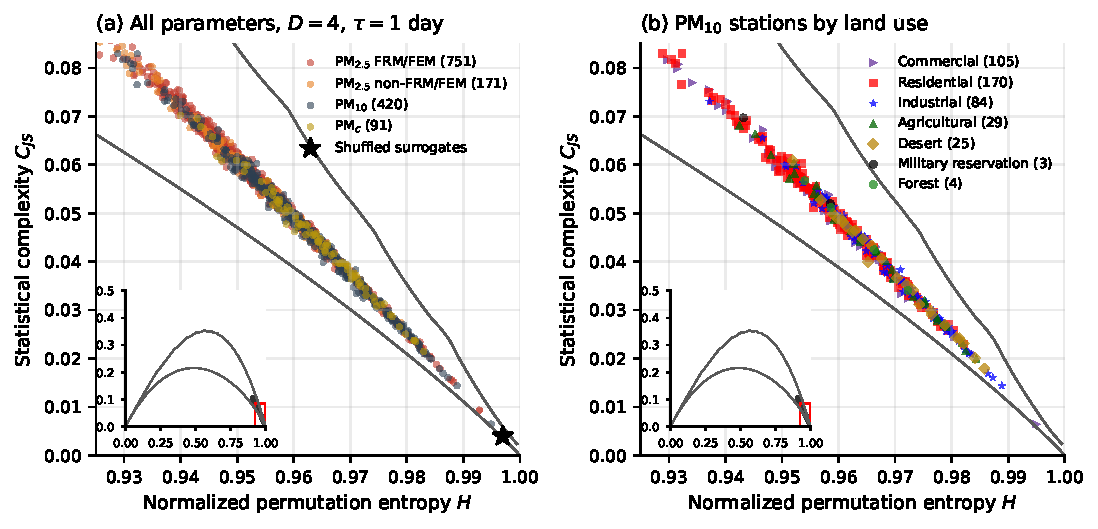
\includegraphics[width=\linewidth]{figs/fig_cecp.pdf}
  \caption{Complexity--entropy causality plane for the full 2023--2025 record of each station ($D=4$, $\tau=1$ day). Grey curves are the minimum and maximum statistical complexity attainable for a given entropy; the insets show the complete plane, with the zoomed region outlined in red. (a) All parameters, with the median of the shuffled surrogates (star). (b) PM$_{10}$ stations colored by land use.}
  \label{fig:cecp}
\end{figure}

The size fractions differ systematically in their ordinal structure. At collocated sites, PM$_{2.5}$ FRM/FEM is more ordered than PM$_{10}$ ($r_{rb}=-0.35$ for $H$, 242 sites) and much more ordered than PM$_{c}$ ($r_{rb}=-0.69$, 91 sites), and PM$_{10}$ is more ordered than PM$_{c}$ ($r_{rb}=-0.61$, 78 sites; all $p<0.001$), whereas the two PM$_{2.5}$ methods are indistinguishable ($r_{rb}=-0.01$, 22 sites). The ordering PM$_{2.5}<$ PM$_{10}<$ PM$_{c}$ in permutation entropy is physically meaningful: fine particles are dominated by regionally mixed secondary aerosol and long-range transport, which vary smoothly with synoptic meteorology, whereas coarse particles respond to local, intermittent resuspension and wind events that decorrelate quickly. Within seasonal windows ($D=3$), the same ordering appears with smaller effect sizes and remains significant after Holm correction only for the PM$_{10}$--PM$_{c}$ contrast ($r_{rb}=-0.48$; Table~\ref{tab:complexity_tests}), where the coarse fraction is also more skewed ($r_{rb}=-0.49$ for skewness). Figure~\ref{fig:complexity_structure}a shows that the metrics capture partly distinct properties: with $D=3$, $H$ and $C_{JS}$ are perfectly redundant ($\rho=-1.00$), so that the complexity--entropy plane collapses to a curve; SVD entropy and the Higuchi dimension are strongly related ($\rho=0.71$), skewness and kurtosis almost interchangeable ($\rho=0.96$), and sample entropy decreases with tail weight ($\rho=-0.59$ with skewness), whereas ordinal and amplitude-based irregularity are nearly independent ($\rho=0.11$ between $H$ and sample entropy). Reporting a subset of non-redundant metrics, as done below, avoids double counting the same information.

\subsection{Seasonal and land-use structure of PM dynamics}

Seasonality is the main source of variation in the dynamics of the fine fraction (Fig.~\ref{fig:complexity_seasonal} and Table~\ref{tab:complexity_tests}). For PM$_{2.5}$ FRM/FEM, summer windows are smoother and more persistent than winter windows, with lower sample entropy (median 1.36 versus 1.71), lower SVD entropy (0.922 versus 0.956), and lower Higuchi dimension (1.79 versus 1.88; Kendall's $W=0.19$--$0.32$), and they are also more heavy-tailed (excess kurtosis 3.36 versus 1.06). The combination of smooth background variability and rare, intense excursions is the signature of multi-day episodes, such as heat-driven secondary formation and wildfire smoke; the latter was exceptional during the 2023 Canadian fire season, which affected large parts of the United States \citep{Wang2024, Butler2024}. The non-FRM/FEM PM$_{2.5}$ series reproduce the same pattern, with an even stronger seasonal contrast in sample entropy ($W=0.34$). PM$_{10}$ and PM$_{c}$ show weaker seasonality ($W\le0.22$), with the smoothest trajectories in autumn and no significant seasonal change in sample entropy.

\begin{figure}[!htbp]
  \centering
  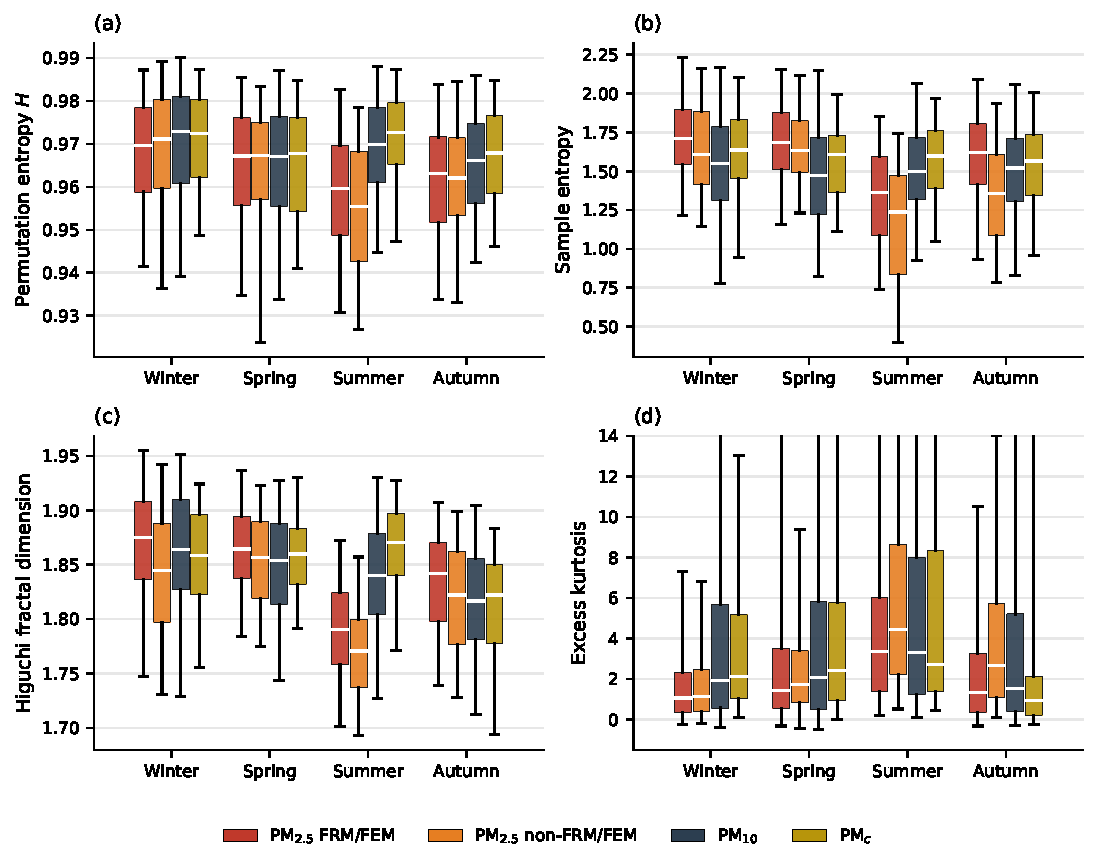
\includegraphics[width=0.92\linewidth]{figs/fig_complexity_seasonal.pdf}
  \caption{Seasonal distribution of station-median complexity metrics by parameter: (a) permutation entropy ($D=3$), (b) sample entropy, (c) Higuchi fractal dimension, and (d) excess kurtosis. Boxes show interquartile ranges and whiskers the 5th--95th percentiles; in panel (d) the axis is truncated at 14.}
  \label{fig:complexity_seasonal}
\end{figure}

\begin{table*}[!htbp]
\centering
\footnotesize
\caption{Effect sizes for the temporal-complexity metrics: Kendall's $W$ for the seasonal contrast within stations (Friedman test), $\varepsilon^2$ for the land-use contrast among station medians (Kruskal--Wallis test), and the matched-pairs rank-biserial correlation $r_{rb}$ for collocated size fractions (Wilcoxon signed-rank test; negative values indicate lower values in the first fraction). Window-level metrics with $D=3$. Holm-adjusted significance within each family: $^{*}p<0.05$, $^{**}p<0.01$, $^{***}p<0.001$.}
\label{tab:complexity_tests}
\setlength{\tabcolsep}{4pt}
\begin{tabular}{lccccccc}
\toprule
 & \multicolumn{3}{c}{\textbf{Seasonality ($W$)}} & \multicolumn{2}{c}{\textbf{Land use ($\varepsilon^2$)}} & \multicolumn{2}{c}{\textbf{Paired fractions ($r_{rb}$)}} \\
\cmidrule(lr){2-4}\cmidrule(lr){5-6}\cmidrule(lr){7-8}
\textbf{Metric} & \textbf{\makecell{PM$_{2.5}$\\FRM/FEM}} & \textbf{PM$_{10}$} & \textbf{PM$_{c}$} & \textbf{\makecell{PM$_{2.5}$\\FRM/FEM}} & \textbf{PM$_{10}$} & \textbf{\makecell{PM$_{2.5}$ vs\\PM$_{10}$}} & \textbf{\makecell{PM$_{10}$ vs\\PM$_{c}$}} \\
\midrule
$H$ & 0.064$^{***}$ & 0.036$^{***}$ & 0.060$^{**}$ & 0.008 & 0.127$^{***}$ & $-0.17$ & $-0.48^{**}$ \\
Sample entropy & 0.194$^{***}$ & 0.005 & 0.018 & 0.036$^{**}$ & 0.125$^{***}$ & $+0.12$ & $+0.22$ \\
SVD entropy & 0.319$^{***}$ & 0.118$^{***}$ & 0.169$^{***}$ & 0.014 & 0.143$^{***}$ & $-0.38^{***}$ & $-0.37$ \\
Higuchi dimension & 0.318$^{***}$ & 0.096$^{***}$ & 0.215$^{***}$ & 0.010 & 0.129$^{***}$ & $-0.14$ & $-0.28$ \\
$D_2$ & 0.136$^{***}$ & 0.069$^{***}$ & 0.097$^{***}$ & 0.034$^{**}$ & 0.043 & $-0.32^{***}$ & $+0.14$ \\
Excess kurtosis & 0.103$^{***}$ & 0.039$^{***}$ & 0.089$^{***}$ & 0.047$^{***}$ & 0.128$^{***}$ & $-0.09$ & $-0.39$ \\
\bottomrule
\end{tabular}
\end{table*}

Land use, in contrast, has almost no influence on PM$_{2.5}$ dynamics but a moderate influence on PM$_{10}$ dynamics (Fig.~\ref{fig:complexity_landuse}). For PM$_{2.5}$ FRM/FEM, the land-use effect sizes are negligible to small ($\varepsilon^2\le0.047$), and the largest of them involve the tail statistics, with heavier tails at agricultural and forest sites (median kurtosis 2.2 and 2.6 versus 1.0--1.5 elsewhere), consistent with episodic smoke and secondary aerosol events in rural regions. For PM$_{10}$, land use explains 13--15\% of the rank variance of the ordinal, amplitude, and tail metrics ($\varepsilon^2=0.125$--$0.147$; 0.043 for $D_2$). Desert, industrial, and agricultural monitors, most of them rural, combine higher permutation entropy (0.971--0.976 versus 0.966--0.967 at commercial and residential sites) with lower sample entropy (1.20 at desert sites versus 1.55) and much heavier tails (median excess kurtosis 7.8 at desert sites versus 1.5--1.6). The apparent contradiction between ordinal and amplitude-based irregularity is informative: in a series dominated by rare, large dust or resuspension events, the standard deviation is inflated by the bursts, so that the background days fall within the tolerance of sample entropy and look regular, while the order of consecutive days remains almost random. The same contrast appears along the urbanicity gradient, where rural PM$_{10}$ is more random in its ordinal structure and more heavy-tailed than suburban and urban PM$_{10}$ ($\varepsilon^2=0.12$--$0.14$). For PM$_{c}$, the land-use contrasts are not significant, although the small number of non-urban PM$_{c}$ monitors limits this comparison.

\begin{figure}[!htbp]
  \centering
  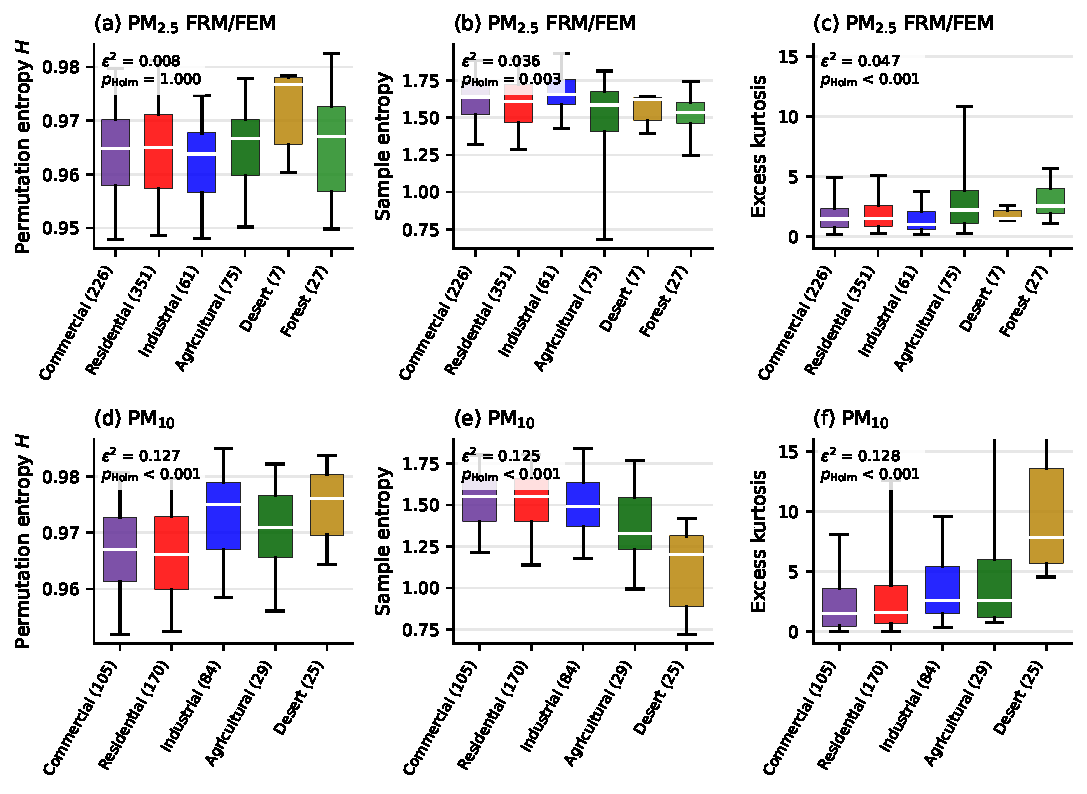
\includegraphics[width=\linewidth]{figs/fig_complexity_landuse.pdf}
  \caption{Station-median complexity metrics by land use for PM$_{2.5}$ FRM/FEM (a--c) and PM$_{10}$ (d--f): permutation entropy ($D=3$), sample entropy, and excess kurtosis. Only land uses with at least five stations are shown (number of stations in parentheses). Boxes show interquartile ranges and whiskers the 5th--95th percentiles. The Kruskal--Wallis effect size $\varepsilon^2$ and the Holm-adjusted $p$-value are given in each panel.}
  \label{fig:complexity_landuse}
\end{figure}

\subsection{Spatial organization of PM dynamics}

Maps of the station-median permutation entropy show coherent regional patterns (Fig.~\ref{fig:complexity_maps}a,b). For PM$_{2.5}$, the most ordered dynamics occur in California and in the southeastern and eastern United States, whereas the most random dynamics occur in the northern Plains and the Mountain West; for PM$_{10}$, the highest entropies concentrate in the arid Southwest and in Wyoming, where many rural industrial and desert monitors are located. Ward clustering of the PM$_{2.5}$ dynamical profiles summarizes this organization (Fig.~\ref{fig:complexity_maps}c and Fig.~\ref{fig:complexity_structure}b). Cluster 1 (120 stations; median longitude $-118.5^\circ$) is concentrated along the Pacific coast, mainly in California, and has the most structured dynamics ($H=0.958$, $C_{JS}=0.039$) and the smoothest trajectories (SVD entropy 0.913, Higuchi dimension 1.79); cluster 2 (134 stations; $-98.5^\circ$) groups the northern Plains, the Mountain West, the upper Midwest, and southern Florida and has the most random ordinal dynamics ($H=0.969$, $C_{JS}=0.029$) together with the lowest sample entropy (1.44); and cluster 3 (497 stations; $-86.1^\circ$) covers most of the East and the Gulf coast and has the highest sample entropy (1.67). The partition is only moderately separated (silhouette width 0.22 for $k=3$; median adjusted Rand index of 0.40 between the full solution and solutions from 80\% subsamples), so the profiles are better described as a continuum with a dominant west--east gradient than as discrete types. In every partition we examined, however, the groups are unrelated to land use (adjusted Rand index $-0.02$; Cram\'er's $V=0.13$) and to location setting (adjusted Rand index 0.00; $V=0.08$), whereas they differ strongly in longitude (Kruskal--Wallis $H=173$, $p<0.001$). PM$_{2.5}$ dynamics are therefore organized by regional meteorology and source mixtures rather than by the local land-use label of the monitor. The persistence of station rankings between years is moderate (Spearman $\rho=0.17$--$0.41$ for PM$_{2.5}$ and $0.23$--$0.53$ for PM$_{10}$, highest for the Higuchi dimension of PM$_{10}$), which indicates that interannual variability, including the 2023 smoke episodes, is an important component of the dynamics at individual sites.

\begin{figure}[!htbp]
  \centering
  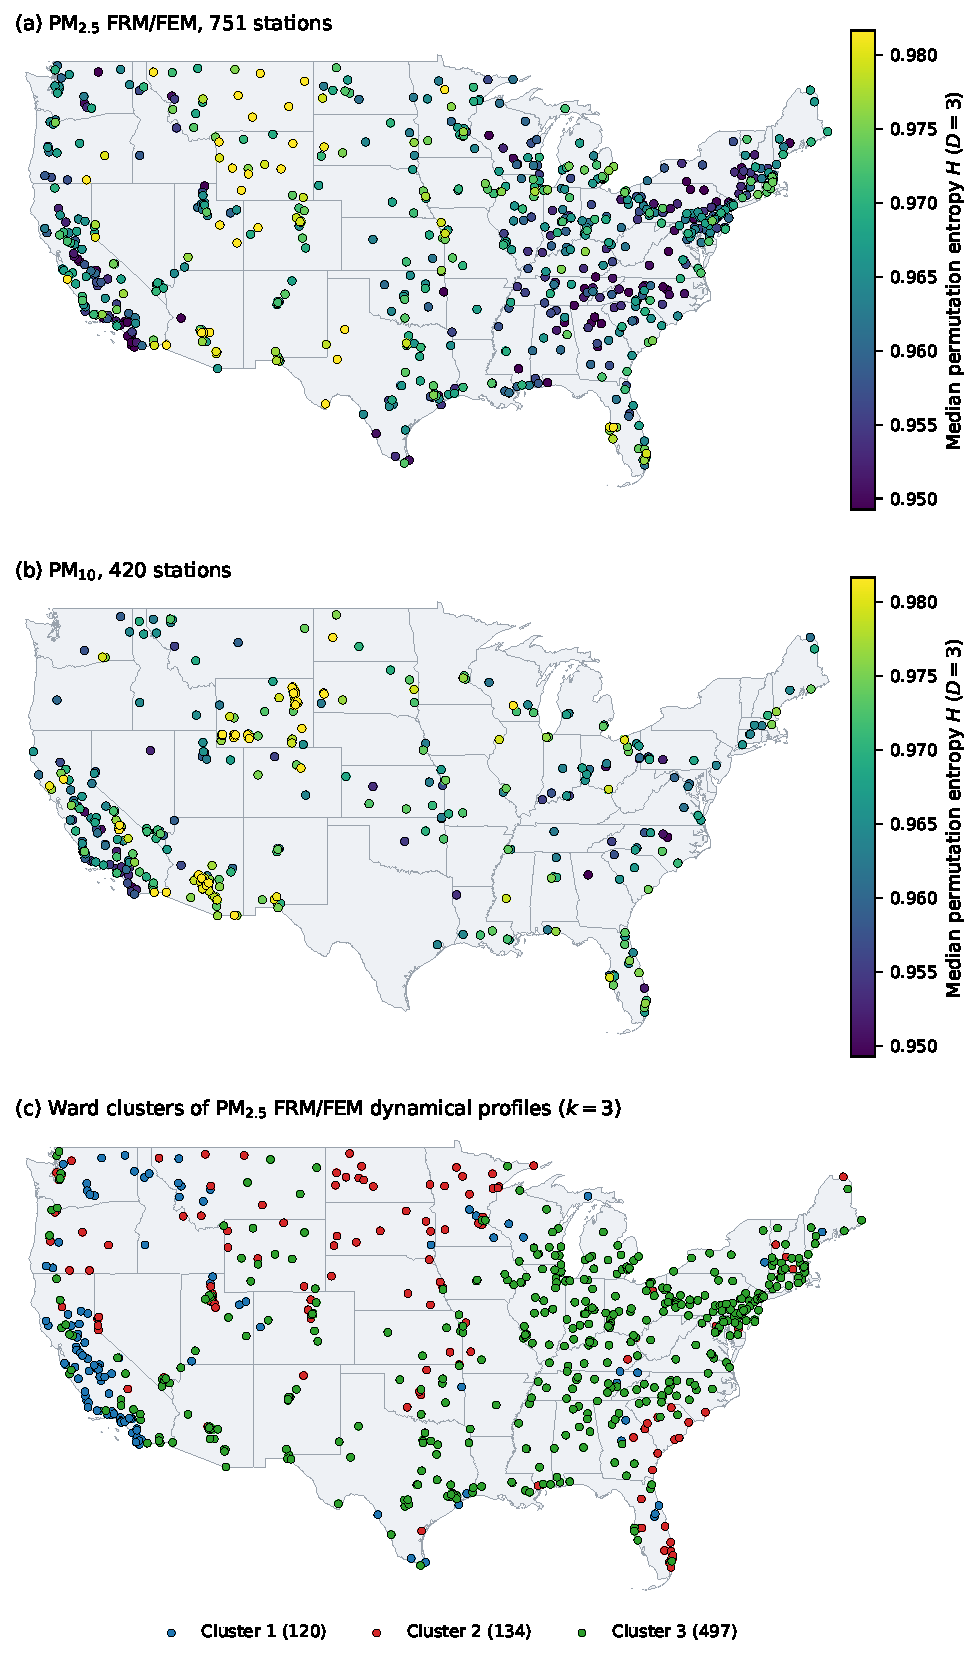
\includegraphics[width=\linewidth,height=0.74\textheight,keepaspectratio]{figs/fig_complexity_maps.pdf}
  \caption{Spatial organization of PM dynamics. (a) Station-median permutation entropy ($D=3$) of PM$_{2.5}$ FRM/FEM and (b) of PM$_{10}$, on a common color scale (5th--95th percentiles). (c) Ward clusters ($k=3$) of the standardized dynamical profiles (permutation entropy, sample entropy, SVD entropy, and Higuchi dimension) of PM$_{2.5}$ FRM/FEM stations, numbered from west to east.}
  \label{fig:complexity_maps}
\end{figure}

\begin{figure}[!htbp]
  \centering
  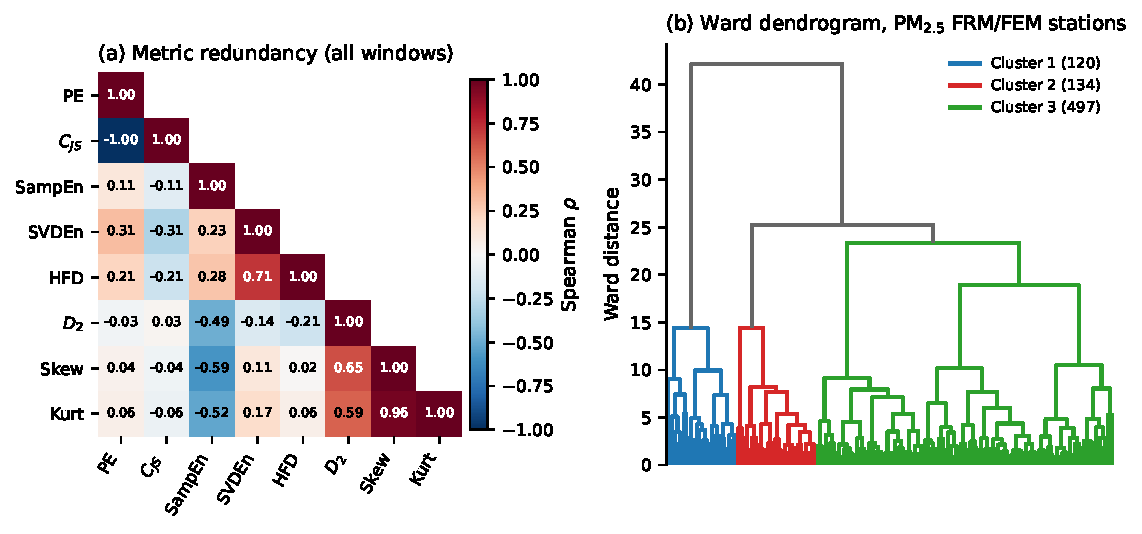
\includegraphics[width=\linewidth]{figs/fig_complexity_structure.pdf}
  \caption{(a) Spearman correlations among the complexity metrics across all season--year windows (PE: permutation entropy; $C_{JS}$: statistical complexity; SampEn: sample entropy; SVDEn: SVD entropy; HFD: Higuchi fractal dimension; $D_2$: correlation dimension; Skew: skewness; Kurt: excess kurtosis). (b) Ward dendrogram of the PM$_{2.5}$ FRM/FEM stations, with the three clusters mapped in Fig.~\ref{fig:complexity_maps}c.}
  \label{fig:complexity_structure}
\end{figure}

\subsection{Linking fine dominance and temporal dynamics}

The two layers of the analysis are related at the station level (Table~\ref{tab:link} and Fig.~\ref{fig:fdi_complexity_link}). Stations with higher mean FDI have more structured PM$_{2.5}$ dynamics, with lower full-period permutation entropy ($\rho_s=-0.31$) and higher statistical complexity ($\rho_s=0.33$), and less bursty PM$_{10}$, with lower skewness ($\rho_s=-0.32$) and kurtosis ($\rho_s=-0.35$) and higher sample entropy ($\rho_s=0.33$). These associations persist after controlling for latitude and longitude ($|\text{partial }\rho_s|=0.24$--$0.39$), so they are not a by-product of the regional gradients described above. Fine-dominated regimes therefore combine a larger share of fine particles with smoother, more persistent fine-particle dynamics and a PM$_{10}$ signal without large coarse bursts, whereas coarse-dominated regimes combine a lower FDI with intermittent, heavy-tailed PM$_{10}$ variability. The size partition and the temporal dynamics are thus two complementary expressions of the same source regime, and their joint use separates sites that a single ratio would treat as equivalent.

\begin{table}[!htbp]
\centering
\footnotesize
\caption{Spearman correlations between the station mean FDI and the station-median complexity metrics of the collocated PM$_{2.5}$ FRM/FEM and PM$_{10}$ series (240 stations), and partial correlations controlling for latitude and longitude. $^{\dagger}$Holm-adjusted $p<0.05$.}
\label{tab:link}
\begin{tabular}{lcccc}
\toprule
 & \multicolumn{2}{c}{\textbf{PM$_{2.5}$ FRM/FEM}} & \multicolumn{2}{c}{\textbf{PM$_{10}$}} \\
\cmidrule(lr){2-3}\cmidrule(lr){4-5}
\textbf{Metric} & \textbf{$\rho_s$} & \textbf{Partial $\rho_s$} & \textbf{$\rho_s$} & \textbf{Partial $\rho_s$} \\
\midrule
$H$ ($D=4$, full period) & $-0.31^{\dagger}$ & $-0.34$ & $-0.14$ & $-0.27$ \\
$C_{JS}$ ($D=4$, full period) & $+0.33^{\dagger}$ & $+0.34$ & $+0.17$ & $+0.29$ \\
Sample entropy & $+0.21^{\dagger}$ & $+0.19$ & $+0.33^{\dagger}$ & $+0.24$ \\
SVD entropy & $-0.05$ & $-0.37$ & $-0.24^{\dagger}$ & $-0.45$ \\
Higuchi fractal dimension & $+0.10$ & $-0.29$ & $-0.11$ & $-0.40$ \\
Skewness & $-0.04$ & $-0.21$ & $-0.32^{\dagger}$ & $-0.39$ \\
Excess kurtosis & $-0.11$ & $-0.26$ & $-0.35^{\dagger}$ & $-0.37$ \\
\bottomrule
\end{tabular}
\end{table}

\begin{figure}[!htbp]
  \centering
  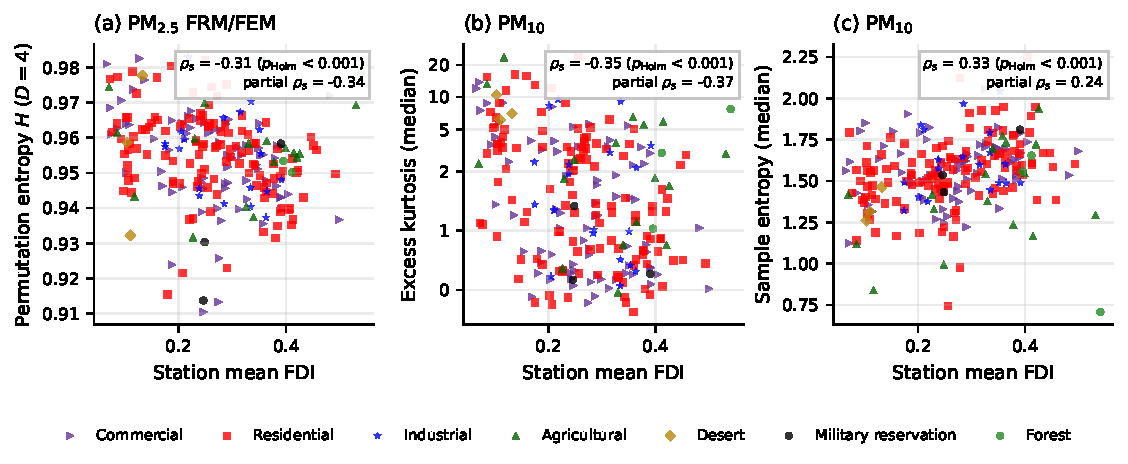
\includegraphics[width=\linewidth]{figs/fig_fdi_complexity_link.pdf}
  \caption{Station mean FDI versus (a) the full-period permutation entropy of PM$_{2.5}$ FRM/FEM ($D=4$), (b) the median excess kurtosis of PM$_{10}$ (symmetric logarithmic axis), and (c) the median sample entropy of PM$_{10}$, for the 240 stations of the fine--coarse network, colored by land use. Each panel reports the Spearman correlation with its Holm-adjusted $p$-value and the partial correlation controlling for latitude and longitude.}
  \label{fig:fdi_complexity_link}
\end{figure}

\subsection{Interpretability, implications, and limitations}

The Fine Dominance Index is interpretable by design. Because it is a bounded, convex transformation of PM$_{2.5}$/PM$_{10}$, larger values correspond to stronger fine-particle dominance, typically associated with combustion and secondary aerosol, while smaller values indicate coarse dust or resuspension. The composite IFS standardizes cell-level summaries into an integrated fingerprint for ranking, without replacing the physically meaningful FDI, and the complexity layer adds information that neither index contains: whether the concentrations of a given fraction evolve smoothly or intermittently. In practice, we recommend reporting the ranked IFS for prioritization, the FDI mean with its station-block interval for interpretation, and, for monitors with suspected coarse influence, the permutation entropy and kurtosis of PM$_{10}$ as indicators of episodic coarse sources.

Several limitations should be noted. Land-use labels and location settings are categorical proxies that cannot capture within-class heterogeneity, proximity to specific sources, or micro-siting effects, and the regulatory network is not a random sample of U.S. environments: desert, forest, and military reservation monitors are few in the fine--coarse network, so the corresponding cells are flagged as thin, and the coarse-dominated regime is best documented by the PM$_{10}$ complexity network. The indices rely on mass concentrations only and do not resolve chemical composition, hygroscopic growth, or aerosol acidity. PM$_{2.5}$ and PM$_{10}$ are measured by different instruments, so that their ratio inherits instrumental uncertainty, and the 1\,\textmu g\,m$^{-3}$ resolution of PM$_{10}$ creates ties that we resolved at random. Seasonal windows of about 90 days limit the embedding dimension of ordinal analyses ($D=3$ within seasons) and constrain the correlation dimension, which is bounded by the embedding dimension of 2 and should be read as a low-dimensional geometric descriptor rather than as an estimate of an attractor dimension. Finally, seasons are defined climatologically and meteorological covariates were not modeled, so that the interpretation of seasonal and regional contrasts in terms of boundary-layer dynamics, smoke, and dust remains inferential.

Despite these caveats, the convergence of distributional evidence, cell-wise fingerprints, station-level tests, and temporal-complexity metrics supports a consistent message: the fine--coarse partition of U.S. particulate matter is controlled first by season and region and only secondarily by land use, and coarse-dominated regimes are characterized as much by the intermittency of their dynamics as by their mass partition. A compact set of complementary metrics, namely the FDI at the sample level, cell-wise summaries with uncertainty, a standardized composite index, and a few non-redundant complexity descriptors, yields a reproducible, source-informed fingerprint that is stable to reasonable modeling choices and directly usable for season- and context-specific air-quality management.

\section{Conclusions}\label{sec:conclusions}

Relying on a single PM$_{2.5}$/PM$_{10}$ ratio or on fixed thresholds is insufficient to separate particulate regimes across heterogeneous U.S. contexts. By combining a bounded, sample-level Fine Dominance Index, cell-wise seasonal fingerprints with station-block uncertainty, station-level nonparametric contrasts, and a temporal-complexity layer, we obtain a compact and interpretable characterization of fine versus coarse dominance for 2023--2025. Fine dominance is primarily seasonal: it peaks in winter at most monitors, and the robust hotspots are winter cells in suburban and urban built environments, whereas coarse dominance prevails at rural industrial sites outside winter and at the few desert monitors. Once pseudo-replication is avoided, land-use differences within a setting are mostly small, with the exception of fine-dominated forest sites and suburban industrial sites.

Daily PM concentrations behave as high-entropy, correlated-noise processes that are nevertheless significantly more ordered than shuffled surrogates. Ordinal entropy increases from PM$_{2.5}$ to PM$_{10}$ to PM$_{c}$, summer fine-particle dynamics are smoother but more heavy-tailed, and land use shapes the dynamics of PM$_{10}$, with intermittent, heavy-tailed variability at desert, industrial, and agricultural sites, but not those of PM$_{2.5}$, which vary mainly with geography. Fine-dominated stations display more structured PM$_{2.5}$ and less bursty PM$_{10}$ dynamics, which shows that mass partition and temporal dynamics are complementary signatures of the same source regimes. Sensitivity analyses on index weights, completeness thresholds, quality-control rules, thin-cell criteria, and individual years indicate that the qualitative hierarchy is stable, although the exact membership of the ranked tables depends on how sparse cells are treated and on the year considered.

Practically, the findings support season- and context-specific air-quality management: wintertime mitigation of combustion and secondary fine aerosol in built environments, and abatement of intermittent coarse sources, such as unpaved roads, construction, mining, and exposed soils, where PM$_{10}$ dynamics are bursty. Future work should integrate chemical speciation and receptor models to validate the fingerprints; incorporate meteorological covariates, boundary-layer data, and smoke and dust event flags to attribute seasonal and regional contrasts; expand coverage for sparse classes such as desert, forest, and military areas; analyze hourly data, which would allow higher embedding dimensions and multiscale complexity measures; extend the temporal scope to test the persistence of the fingerprints; and package the workflow into an operational tool that updates automatically from EPA AirData for routine screening and policy support.

\section*{Data and code availability}
All raw data are openly available from the U.S. EPA AirData pre-generated daily summary archives for 2023--2025 (\url{https://aqs.epa.gov/aqsweb/airdata/download_files.html}). The analysis pipeline, which downloads the data, applies the screening and quality-control rules, and reproduces every table and figure of this article, is publicly available at \url{https://github.com/IsabellaArrieta/atmospheric-pollutants-analysis}.

\section*{Acknowledgments}
We gratefully acknowledge the U.S. Environmental Protection Agency (EPA) for maintaining and openly publishing the AirData/AQS archives. The clarity of documentation, consistent data formatting, and long-term stewardship of these datasets make large-scale, reproducible analyses like this one possible. Any opinions, findings, and conclusions or recommendations expressed in this work are those of the authors and do not necessarily reflect the views of the EPA.

\section*{Declaration of competing interest}
The authors declare that they have no known competing financial interests or personal relationships that could have appeared to influence the work reported in this paper.

\section*{Declaration of generative AI and AI-assisted technologies in the manuscript preparation process}
During the preparation of this work the authors used Claude (Anthropic) to assist with code review, the reanalysis scripts, and language editing. After using this tool, the authors reviewed and edited the content as needed and take full responsibility for the content of the published article.

\printcredits

%% Loading bibliography style file
%\bibliographystyle{model1-num-names}
\bibliographystyle{cas-model2-names}

% Loading bibliography database
\bibliography{cas-refs}


\end{document}
